% ------------------------------------------------------------------
%
% pdflatex gbem-assembly-jfe.tex
% bibtex gbem-assembly-jfe
% xpdf gbem-assembly-jfe.pdf &
%
%%%%%%%%%%%%%%%%%%%%%%%%%%% asme2ej.tex %%%%%%%%%%%%%%%%%%%%%%%%%%%%%%%
% Template for producing ASME-format journal articles using LaTeX    %
% Written by   Harry H. Cheng, Professor and Director                %
%              Integration Engineering Laboratory                    %
%              Department of Mechanical and Aeronautical Engineering %
%              University of California                              %
%              Davis, CA 95616                                       %
%              Tel: (530) 752-5020 (office)                          %
%                   (530) 752-1028 (lab)                             %
%              Fax: (530) 752-4158                                   %
%              Email: hhcheng@ucdavis.edu                            %
%              WWW:   http://iel.ucdavis.edu/people/cheng.html       %
%              May 7, 1994                                           %
% Modified: February 16, 2001 by Harry H. Cheng                      %
% Modified: January  01, 2003 by Geoffrey R. Shiflett                %
% Use at your own risk, send complaints to /dev/null                 %
%%%%%%%%%%%%%%%%%%%%%%%%%%%%%%%%%%%%%%%%%%%%%%%%%%%%%%%%%%%%%%%%%%%%%%
% use twocolumn and 10pt options with the asme2ej format
%%% \documentclass[twocolumn,10pt,final]{asme2ej}
  \documentclass[oneside,onecolumn,10pt,final]{asme2ej}
%%\documentclass[oneside,twocolumn,10pt,final]{asme2ej}
%%%
%%% \usepackage{epsfig} %% for loading postscript figures
%%%
% ..................................................................
%  The class has several options
%  onecolumn/twocolumn - format for one or two columns per page
%  10pt/11pt/12pt - use 10, 11, or 12 point font
%  oneside/twoside - format for oneside/twosided printing
%  final/draft - format for final/draft copy
%  cleanfoot - take out copyright info in footer leave page number
%  cleanhead - take out the conference banner on the title page
%  titlepage/notitlepage - put in titlepage or leave out titlepage
%  
%  The default is oneside, onecolumn, 10pt, final
%
% ------------------------------------------------------------------
% External packages
% -----------------------------------------------------------------
\usepackage{amsmath,amsfonts,amssymb,mathtools}
\usepackage{mathtools}  % 
\usepackage{bm}         % general bold symbols
% ------------------------------------------------------------------
\usepackage{ifthen}     % conditional compilation
\usepackage{color,soul} % uso: \hl {texto}
\usepackage{cancel}     % para tachar \hl {{\cancel {xx}}}
% -----------------------------------------------------------------
\usepackage{sistyle}   % an intermediate package for SI units
%usepackage{siunitx}   % better package that collects several ones
% -----------------------------------------------------------------
% Itemiza
\usepackage{paralist}   % para {compactitem}
\usepackage{enumitem}   % para {itemize}[noitemsep]
%\begin{compactitem}
%\end{compactitem}
% -----------------------------------------------------------------
%\usepackage[margin=1cm]{geometry}
%\usepackage{tabularx}
%\usepackage[figuresright]{rotating} % sidewaystable
\usepackage{rotating}
\usepackage{adjustbox}
\usepackage{booktabs}
\usepackage{xspace}
% -----------------------------------------------------------------
% Interlineado
% http://tex.stackexchange.com/questions/819/double-line-spacing
%\def\baselinestretch{1.0} %% COMENTAR
% -----------------------------------------------------------------
\usepackage{setspace}
 \doublespacing
% ..................................................................
% http://tex.stackexchange.com/questions/164140/how-to-tell-latex
%  -to-place-all-figures-at-the-end-of-pdf-file
 \usepackage[nomarkers]{endfloat}             % journals mode
%\usepackage[nomarkers,figuresonly]{endfloat} % journals mode
% -----------------------------------------------------------------
\usepackage{booktabs}  % better thickness and spacing around rules
\usepackage{multirow}  %
%\usepackage[tableposition=top]{caption} % more spacing caption/table
% ------------------------------------------------------------------
% User packages
\usepackage{klaves}
%
% ------------------------------------------------------------------
% Bold calligraphic typeface, e.g. see
% https://tex.stackexchange.com/questions/2783/bold-calligraphic-typeface
\DeclareMathAlphabet\mathbfcal{OMS}{cmsy}{b}{n}
%
% ------------------------------------------------------------------
% tabular columns wide control
% https://tex.stackexchange.com/questions/38272/tabular-columns-too-wide
\setlength{\tabcolsep}{4pt}
% ------------------------------------------------------------------
% Otro recurso para anotaciones arriba/debajo de las ecuaciones
\usepackage{stackengine}
\stackMath
% ------------------------------------------------------------------
% Colores: ver listado en Latex Color, http://latexcolor.com/
% ------------------------------------------------------------------
% Colores: ver listado en Latex Color, http://latexcolor.com/
\definecolor{airforceblue}{rgb}{0.36,0.54,0.66}%Air Force blue #5D8AA8
\definecolor{americanrose}{rgb}{1.00,0.01,0.24}%American rose #FF033E
\definecolor{arylideyellow}{rgb}{0.91,0.84,0.42}%Arylide yellow	#E9D66B 	
\definecolor{asparagus}{rgb}{0.53,0.66,0.42}%Asparagus #87A96B
\definecolor{atomictangerine}{rgb}{1.0,0.6,0.4}%Atomic tangerine#FF9966
\definecolor{cadmiumyellow}{rgb}{1.0,0.96,0.0}%Cadmium Yellow #FFF600
\definecolor{canaryyellow}{rgb}{1.0,0.94,0.0}%Canary yellow #FFEF00
\definecolor{chromeyellow}{rgb}{1.0,0.65,0.0}%Chrome yellow #FFA700
\definecolor{cyan}{rgb}{0.0,1.0,1.0}%Cyan #00FFFF
\definecolor{earthyellow}{rgb}{0.88,0.66,0.37}%Earth yellow #E1A95F
\definecolor{electricyellow}{rgb}{1.0,1.0,0.0}%Electric yellow %#FFFF00
\definecolor{etonblue}{rgb}{0.59,0.78,0.64}%Eton blue #96C8A2
\definecolor{lightapricot}{rgb}{0.99,0.84,0.69}%Lightapricot #FDD5B1
\definecolor{lightcornflowerblue}{rgb}{0.6,0.81,0.93} % #93CCEA
\definecolor{lightcyan}{rgb}{0.88,1.0,1.0}%Light cyan #E0FFFF
\definecolor{lightkhaki}{rgb}{0.94,0.9,0.55}%Lightkhaki #F0E68C
\definecolor{lightsalmon}{rgb}{1.0,0.63,0.48}%Light salmon #FFA07A
\definecolor{naplesyellow}{rgb}{0.98,0.85,0.37}%Naples yellow #FADA5E
\definecolor{palepink}{rgb}{0.98,0.85,0.87}%Pale pink #FADADD
\definecolor{white}{rgb}{1.0,1.0,1.0}%White #FFFFFF
\definecolor{wildstrawberry}{rgb}{1.0,0.26,0.64}%Wild Strawberry#FF43A4
\definecolor{wildwatermelon}{rgb}{0.99,0.42,0.52}%Wild Watermelon#FC6C85
\definecolor{yellow}{rgb}{1.0,1.0,0.0}%Yellow #FFFF00
% ------------------------------------------------------------------
\DeclareRobustCommand{\ha}[1]{{\sethlcolor{lightkhaki}\hl{#1}}}
\DeclareRobustCommand{\hb}[1]{{\sethlcolor{americanrose}\hl{#1}}}
\DeclareRobustCommand{\hc}[1]{{\sethlcolor{atomictangerine}\hl{#1}}}
\DeclareRobustCommand{\hd}[1]{{\sethlcolor{blue}\hl{#1}}}
\DeclareRobustCommand{\he}[1]{{\sethlcolor{lightapricot}\hl{#1}}}
\DeclareRobustCommand{\hf}[1]{{\sethlcolor{green}\hl{#1}}} 
\DeclareRobustCommand{\hg}[1]{{\sethlcolor{palepink}\hl{#1}}}
\DeclareRobustCommand{\hh}[1]{{\sethlcolor{wildstrawberry}\hl{#1}}}
\DeclareRobustCommand{\hi}[1]{{\sethlcolor{lightsalmon}\hl{#1}}}
\DeclareRobustCommand{\hy}[1]{{\sethlcolor{yellow}\hl{#1}}}
% -----------------------------------------------------------------
% comentar o descomentar para ver o no ver los cambios:
%\DeclareRobustCommand{\ha}[1]{{\sethlcolor{white}\hl{#1}}}
%\DeclareRobustCommand{\he}[1]{{\sethlcolor{white}\hl{#1}}}
%\DeclareRobustCommand{\hf}[1]{{\sethlcolor{white}\hl{#1}}}
%\DeclareRobustCommand{\hg}[1]{{\sethlcolor{white}\hl{#1}}}
%\DeclareRobustCommand{\hi}[1]{{\sethlcolor{white}\hl{#1}}}
%\DeclareRobustCommand{\hh}[1]{{\sethlcolor{white}\hl{#1}}}
%\DeclareRobustCommand{\hy}[1]{{\sethlcolor{white}\hl{#1}}}
% -----------------------------------------------------------------
% end
% ------------------------------------------------------------------

% -----------------------------------------------------------------
% a user counter is defined
\newcounter{tema}
\setcounter{tema}{1} % 1: pdlatex, 2: latex ASME, 3: count words
% -----------------------------------------------------------------
% for loading postscript or pdf figures
\ifthenelse{\value{tema}=1}{% begin tema 1
  \usepackage{graphicx} % tema 1 formato IJCFD 
}{}% end tema 1
%
\ifthenelse{\value{tema}=2}{% begin tema 2
 \usepackage{epsfig}    % tema 2 formato ASME
}{}% end tema 2

% ------------------------------------------------------------------
\title{%
   An improved assembling algorithm in boundary elements with 
   Galerkin weighting applied to three-dimensional Stokes flows
}%end figures

%%% first author
\author{\hspace{-2.5cm}Sofia Sarraf%
  \thanks{%
    CONICET: Consejo Nacional de Investigaciones %
             Cient\'{\i}ficas y T\'ecnicas,      %
    UNCo:    Universidad Nacional del Comahue,   %
    \hy {IITCI: Instituto de Investigaci\'on en  %
                Tecnolog\'{\i}as y Ciencias de   %
                la Ingenier\'{\i}a.}
         } \\
  \affiliation{%
    \hspace{-2.5cm} Associate professor (UNCo)   \\
    \hspace{-2.5cm} Research associate (CONICET) \\
    \hspace{-2.5cm} \hy {IITCI (UNCo-CONICET)} \\ %
    \hspace{-2.5cm} Buenos Aires 1400, (\hy{Q8300IBX})
                    Neuqu\'en, Argentina \\ %
    \hspace{-2.5cm} Email: sofia.sarraf@fain.uncoma.edu.ar %
              }%
}%
% -----------------------------------------------------------------
%%% second author
%%% remove the following entry for single author papers
%%% add more entries for additional authors
%%% Associate professor,graduate Researcher}%
\author{\hspace{2.5cm}Ezequiel L\'opez%
  ~\\
  \affiliation{%
    \hspace{2.5cm} Associate professor (UNCo)   \\
    \hspace{2.5cm} Research associate (CONICET) \\ %
    \hspace{2.5cm} \hy {IITCI (UNCo-CONICET)} \\ %
    \hspace{2.5cm} Buenos Aires 1400, (\hy{Q8300IBX})
                   Neuqu\'en, Argentina \\ %
    \hspace{2.5cm} Email: ezequiel.lopez@fain.uncoma.edu.ar %
              }%
}%
% -----------------------------------------------------------------
%%% third author
%%% remove the following entry for single author papers
%%% add more entries for additional authors
\author{ \hy{Laura Battaglia}, %$^{*}$, %
            Gustavo R\'{\i}os Rodr\'{\i}guez\\ 
  {\tensfb  Jorge D'El\'{\i}a}%
  \thanks{%
      UNL: Universidad Nacional del Litoral,
  \hy{UTN: Universidad Tecnol\'ogica Nacional},
      CIMEC: Centro de Investigaci\'on de M\'etodos Computacionales, 
      corresponding author.} \\ 
      %% Facultad Regional Santa Fe (FRSF) % 
  \affiliation{%
    Associate professors (\hy{UTN}, UNL, and UNL) \\
    Senior Researchers (CONICET) \\
    CIMEC (UNL-CONICET)                       \\
    Predio CONICET-Santa Fe, Colectora RN 168 \\
    El Pozo, Santa Fe (\hy{3000}), Argentina   \\     
    Email: %
    \hy{lbattaglia@santafe-conicet.gob.ar}, %
    gusadrr@santafe-conicet.gov.ar,
    jdelia@intec.unl.edu.ar %
              }%
}

% parametros
%
\newcommand{\rmorinoone}{100-71=29} % 100-71=29 morino-sphere-dgesv r10
\newcommand{\rmorinotwo}{100-53=47} % 100-53=47 morino-sphere-dgesv r31
%
\newcommand{\rstokesone}{100-51=49} % 100-51=49 stokes-sphere-dgesv r10
\newcommand{\rstokestwo}{100-68=32} % 100-68=32 stokes-sphere-dgesv r21
\newcommand{\roscilaone}{100-51=49} % 100-51=49 oscila-sphere-zgesv r10
%
\newcommand{\rstokesoneb}{49} % 100-51=49 stokes-sphere-dgesv r10
\newcommand{\rstokestwob}{32} % 100-68=32 stokes-sphere-dgesv r21
\newcommand{\roscilaoneb}{49} % 100-51=49 oscila-sphere-zgesv r10

% ++++++++++++++++++++++++++++++++++++++++++++++++++++++++++++++++++
\begin{document}

\maketitle    

%%%%%%%%%%%%%%%%%%%%%%%%%%%%%%%%%%%%%%%%%%%%%%%%%%%%%%%%%%%%%%%%%%%%%%
\begin{abstract} {\it %This is the abstract.
  %
  In the Boundary Element Method (BEM), the Galerkin weighting 
  technique allows to obtain numerical solutions of a 
  Boundary Integral Equation (BIE), giving the Galerkin 
  Boundary Element Method (GBEM). 
  %
  In three-dimensional (3D) spatial domains, the nested 
  double surface integration of GBEM leads to a significantly
  larger computational time for assembling the linear system
  than with the standard collocation method.
  %
  \hg {In practice, the} computational time is roughly an order
  of magnitude larger, thus limiting the use of GBEM in 3D
  engineering problems.
  %
  The standard approach for reducing the computational time
  of the linear system assembling is to skip integrations 
  whenever possible.
  %
  In this work, \hg {a modified assembling algorithm for the
  element matrices in GBEM is proposed for solving integral
  kernels that depend on the exterior unit normal}. 
  %
  This algorithm is based on \hg {kernels symmetries at
  the element level and not on the flow nor in the mesh}.
  It is applied to a BIE that models external creeping flows
  around 3D closed bodies using second-order kernels, and it
  is implemented using OpenMP. 
  %
  \hg{For these BIEs, the modified algorithm is on average
  $\rstokestwob$\% faster than the original one.}
  %
\noindent
Keywords: % son las opciones del listado en la ASME
Complex Flows,  
Computational Fluid Dynamics, 
Microfluidics, 
Newtonian Flows 
% %\begin{keywords}
% Keywords (MSC (2010): %
%     76D07  Stokes and related (Oseen, etc.) flows,
%     65N38  Boundary element methods,
%     65D30  Numerical integration. 
% Keywords (PACS (2010):
%     02.70.Pt  Boundary-integral methods,
%     02.70.Dh  Finite-element and Galerkin methods,
%     47.15.G-  Low-Reynolds-number (creeping) flows.
% %\end{keywords}
%
}% italics
\end{abstract}

% ++++++++++++++++++++++++++++++++++++++++++++++++++++++++++++++++++
\section{Introduction}
\label{sec:intro}

%parrafo
\noindent
As is \he {well} known, the Boundary Element Method (BEM) is based 
on the formulation of a boundary value problem of elliptic 
type as a Boundary Integral Equation (BIE) %  
% \citep [e.g. see][]{rf:hackbusch-book,rf:jdelia-ijcfd1}.
% e.g. \cite{rf:hackbusch-book,rf:jdelia-ijcfd1}.
\cite{rf:power-wrobel,rf:jdelia-asmejfe}.
%

%parrafo
\noindent
Two standard discretization procedures of a BIE are the 
point collocation technique\hg{,} and the Galerkin
weighting method (GBEM, Galerkin BEM).
%
Examples of weighted residual techniques in a BIE include 
%
the symmetric boundary element method % 
\cite{rf:terravecchia3}, %%{rf:leonetti-mazza-aristodemo}, 
the symmetric Galerkin boundary element method (SGBEM)%
\cite{rf:zhaoyuan,rf:sgbem-book1,rf:salvadori1}, %% {rf:bonnet0}
and the variational boundary element method %
\cite{rf:alia-souli-erchiqui}, among others.
%
In the case of kernels with a weak singularity, there are 
analytical expressions of the double surface integrals as, 
for instance, the potential integrals in computational 
electromagnetics\hg{,} which are designed for flat triangles
but restricted to kernels with a linear or constant
density layer in the numerator \cite{rf:sievers}.
%
More recently, \hg {Carley} %
\cite{rf:carley-2013} has proposed a method for evaluating
potential integrals on planar triangular elements using a
polar coordinate decomposition, with explicit formulas for
the regular, principal value, and finite part integrals.

%parrafo
\noindent
\hg{In classical formulations of the collocation and the}
Galerkin weighting techniques, every element interacts 
with the others, \hg {leading} to dense influence matrices.
The computation of these matrices involves a cost $O(M^2)$,
where $M$ is the number of degrees of freedom.
%
The influence matrix for each pair of elements in GBEM
requires the computation of double surface interaction
integrals with a weak singularity, which are solved in this
work with an extension of the scheme proposed \hg {by Taylor}
\cite{rf:taylordj1}, where a systematic way for handling 
double surface integrals \hg{over} flat triangular elements
\he {is developed}.
%...................................................................
% referato 20170322
\hy {The strategy is based on a convenient reordering of the
four iterate integrations that moves the weak singularity to
the origin of the four-dimensional Euclidean space and then
systematically applies the Duffy transformation} \cite{rf:taylordj1}, 
\hy {i.e. regularizes the integrand by using polar coordinates. 
Taylor uses a Gauss--Legendre numerical quadrature on three
coordinates and performs an analytic integration in the fourth one}. 
\hy {However, since the Taylor scheme is restricted to wave
propagation kernels in computational electromagnetics, a
modification was proposed in} \cite{rf:jdelia-gbem1,rf:ssarraf-torus},
\hy {where the fourth analytic integration of the Taylor scheme is 
replaced by a numerical quadrature in order to handle kernels with
a weak singularity under a general framework}.

%parrafo
\noindent
The assembly of the system matrix for GBEM is performed 
by means of a double loop over the whole set of elements. 
%
In three-dimensional (3D) spatial domains, this double 
loop leads to a significantly greater computational time
for assembling the linear system than \hg {with the
collocation technique}.
%
\hg{The time ratio needed for assembling the matrix 
with collocation and GBEM is roughly one order of magnitude}. 
This fact has severely limited the use of GBEM in 3D 
engineering problems \cite{rf:iemma}. %,rf:gray-griffith}.
%
The standard approach for reducing the computational time 
in the assembling of the linear system is to avoid integrations 
whenever possible. However this can be difficult to 
perform in mixed BIEs where some kernel components depend  
on the exterior unit normal. % \cite{rf:gray-griffith}.
%
In general, the double loop for the linear system assembly  
can not be eliminated, although it is plausible to 
take advantage of block symmetries at the level of the 
element matrix, which is \hg{computed} as a double surface 
integral where its integrand is a double matrix product.
%
Other relationships \he {between} coefficient matrices in SGBEM for
two-dimensional scalar problems were given in \cite{rf:yu-jam}.
%
\hy{The aim of this work is to propose a strategy able to
reduce the computational time in the assembly stage through
schemes that use the kernel symmetries in GBEM.
In particular, the 3D creeping flow kernel is addressed,
which is used in the modeling of several flow problems
such as micro-electromechanical systems (MEMS) simulation}
\cite{rf:mukherjee-telukunta, rf:enief07-vfachinotti-full},
\hy {peristaltic transport in microfluidic channels}
\cite{rf:bandopadhyay-tripathi-chakraborty,
  rf:tripathi-brushan-anwarbeg,rf:tripathi-yadav-anwarbeg},
\hy {among others}. 
The proposed method is implemented using OpenMP on
a multi-core computer \cite{rf:diaz-caro-ninio}.

%parrafo
\noindent
\hg {The work is organized} as follows. First, the GBEM
technique is reviewed for a BIE of the Fredholm type and
second kind, \hh{with mixed and weakly singular} second-order 
tensor kernels. %% \citep{rf:power-wrobel}, 
%
Then, \hg {due to symmetries of the Green function},
the proposed scheme which takes advantage
of the block symmetries at the element matrix level
is presented.
%
The numerical examples \hg {include flow} problems with
analytic or numerical solutions taken from the literature.
%
% %%%%%%%%%%%%%%%%%%%%%%%%%%%%%%%%%%%%%%%%%%%%%%%%%%%%%%%%%%%%%%%%%%
\begin{figure*}[t]
% ..................................................................
\ifthenelse{\value{tema}=1} {\centerline{%
  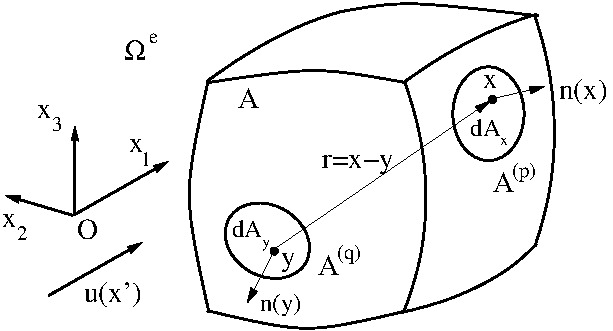
\includegraphics[width=6.5truecm]{./FIG/notatio5-gbem}
  \hspace{40pt}%
  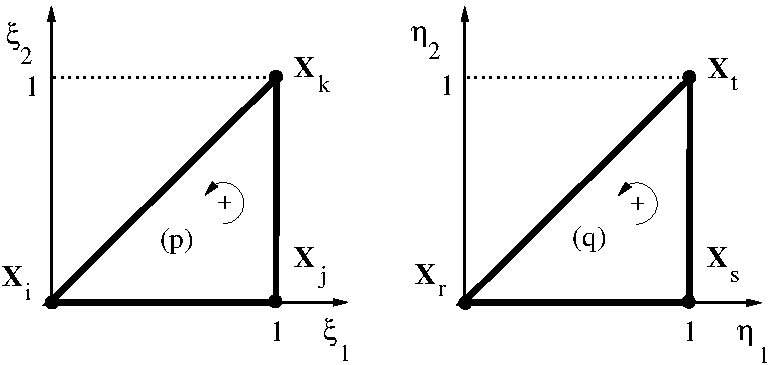
\includegraphics[width=8.0truecm]{./FIG/m-master1}
}}{}% end tema 1
% ..................................................................
\ifthenelse{\value{tema}=2} {\centerline{%
  \psfig{width=6.5truecm,figure=./FIG/notatio5-gbem}
} \vspace{5pt} \centerline{%
  \psfig{width=8.0truecm,figure=./FIG/m-master1}
}}{}% end tema 2
% ..................................................................
\caption{\hg{Left}: a rigid, closed, piecewise
  smooth surface $A$ with an exterior domain $\Omega^e$: %
  field point $\bm {x}$, source point $\bm {y}$, %
  relative position $\bm {r}=\bm {x}-\bm {y}$, %
  unit normals $\bm {n}(\bm {x}), \bm {n}(\bm {y})$,
  and differential areas $\dif A_{\bm {x}}, \dif A_{\bm {y}}$.
  %
  \hg{Right}: master triangles $p$ and $q$ for the simplex
  coordinates}%
\label{fg-notation-gbem}
\end{figure*}
% %%%%%%%%%%%%%%%%%%%%%%%%%%%%%%%%%%%%%%%%%%%%%%%%%%%%%%%%%%%%%%%%%%


% ------------------------------------------------------------------
\section{The Power-Miranda/Hebeker integral formulation}
\label{subsec:power-miranda-hebeker-if}

%parrafo
\noindent
The Power-Miranda/Hebeker integral formulation (or PMH-IF
for short) consists in a BIE without rigid modes for the
Stokes flow around a rigid, closed, piecewise smooth surface
$A$ in $\mathbb{R}^3$, and it can be classified as a 
Completed Indirect Velocity BIE 
(CIV-BIE) \cite{rf:ingber1}, or Completed Double-Layer BIE
(CDL-BIE) \cite{rf:power-wrobel,rf:pozrikidis2}.
%% \cite{rf:karrila-book}. 
%
In this section, Cartesian tensor notation is used, i.e. the
indices $i,j,k$ have the values $1,2,3$ and correspond to the
Cartesian coordinates $(x,y,z)$, respectively.
%
An indirect integral formulation for the Stokes equation
leads to consider %
%
\hg{the single-layer ${\tilde S}_{ij} (\bm{x},\bm{y})$ and 
the double-layer ${\tilde K}_{ij} (\bm{x},\bm{y})$ kernels}. 
%
For the steady flow case these kernels are given by %
\cite{rf:power-wrobel,rf:pozrikidis2}
%
% ..................................................................
\ifthenelse{\value{tema}<3}{% begin tema 3
  \begin{subequations}
  \begin{align}
    %
    {\tilde S}_{ij} (\bm {x},\bm {y}) &= % +
    \frac {1} {8 \pi \mu}
                       \left  [
                         \frac {\delta_{ij}} {r} +
                         \frac {r_i r_j} {r^3}
                         \right ] % \ ;
    \label{eq:stokes0140} \\
    %
    {\tilde K}_{ij} (\bm{x},\bm{y}) & = - \frac {3} {4 \pi}
    \frac {r_i r_j r_k} {r^5} n_k (\bm{y}) % \ ;
    \label{eq:stokes0110}
     %
  \end{align}
  \end{subequations}
%
}{}% end tema 3
% ..................................................................
%
where $\bm {r} = \bm {x} - \bm {y}$ 
and   $ r = \| \bm {x} - \bm {y} \|_2$, 
%
with the integration and field points $\bm{y}=(y_1,y_2,y_3)$ 
and $\bm{x}=(x_1,x_2,x_3)$, respectively
(see Fig.~\ref{fg-notation-gbem}, left),
%
while $n_k=n_k(\bm{y})$ is the unit normal
to the surface $A$ at point $\bm{y}$, 
%
$\delta_{ij}$ is the Kronecker delta,
$\|\cdot\|_2$ is the Euclidean norm for vectors, 
$\mu$ is the dynamic viscosity of the fluid,
and the Einstein summation convention over 
repeated indices is employed. 
%
For \hg {oscillatory} Stokes flow the kernels
\he {adopt} the following expressions \cite{rf:pozrikidis2}
%
% ..................................................................
\ifthenelse{\value{tema}<3}{% begin tema 3
  \begin{subequations}
  \begin{align}
    %
    {\tilde S}_{ij} (\bm {x},\bm {y}) &= 
    \frac {1} {8 \pi \mu}
    \left  [
      \frac {\delta_{ij}} {r} \mathcal {A} (s) +
      \frac {r_ir_j} {r^3} \mathcal {B} (s)
    \right ] % \ ;
    \label{eq:hstokes0100} \\
    %
    {\tilde K}_{ij} (\bm{x},\bm{y}) & = 
    - \frac {1} {4 \pi}
      \biggl \{ % 
      \frac {(\delta_{ij} r_k + \delta_{kj} r_i)} {r^3} c_1 (s)
    + \frac { \delta_{ik} r_j} {r^3} c_2 (s)
    \nonumber \\
    %
    & + \frac {r_i r_j r_k} {r^5} c_3 (s) \biggr \} n_k (\bm {y})
    %
    \label{eq:hstokes0110} %% \\
    %
  \end{align}
  \end{subequations}
  %
}{}% end tema 3
% ..................................................................
%
\hg {in which}
%
% ..................................................................
\ifthenelse{\value{tema}<3}{% begin tema 3
  \begin{subequations}
  \begin{align}
    %
    \mathcal {A} (s) &= 
    2e^{-s} \left (1 + \frac {1} {s} + 
              \frac {1} {s^2} \right ) -
              \frac {2} {s^2} 
    \label{eq:hstokes0112} \\
    %
    \mathcal {B} (s) &= 
      -2e^{-s} \left (1 + \frac {3} {s} + 
            \frac {3} {s^2} \right ) + \frac {6} {s^2} 
    \label{eq:hstokes0114} \\
    %
    c_1 (s) &= e^{-s} (s + 1) - \mathcal {B} (s)
    \label{eq:hstokes0116} \\
    %
    c_2 (s) &= 1 - \mathcal {B} (s)
    \label{eq:hstokes0118} \\
    %
    c_3 (s) &= 5 \mathcal {B} (s) - 2 e^{-s} (s + 1)
    \label{eq:hstokes0120}
    %
  \end{align}
  \end{subequations}
  %
}{}% end tema 3
% ..................................................................
%
\hy{where $ s = r \sqrt {-I \Omega/ \nu} $ is the
non-dimensional distance}, $\Omega = 2 \pi f$ is the
circular frequency of the oscillation, $\nu=\mu/\rho$
\hg {is} the kinematic viscosity of the fluid, and $I$
\hg {is} the imaginary unit, while $f$ is the frequency
in Hz, and $\rho$ is the fluid density.  
%
The PMH-IF uses both single and double layer
densities, and it can be written as \cite{rf:jdelia-gbem2}
%% rf:pozrikidis2 rf:hebeker rf:power-wrobel
%
% ..................................................................
\ifthenelse{\value{tema}<3}{% begin tema 3
  \begin{equation}
    %% g_i (\bm {x})
    u_i (\bm {x}) =  \int_A  \left  [
    {\tilde K}_{ij} \psi_j (\bm {x}) - 
    {\tilde H}_{ij} \psi_j (\bm {y})
                          \right ] \dif A_{\bm {y}},
    \quad \mbox {for all $\bm{x} \in A$}
    \label{eq:stokes0160}
  \end{equation}  
  %
}{}% end tema 3
% ..................................................................
%
where $\psi_j (\bm{x})$ is the double-layer surface density, 
and $u_i (\bm{x})$ is the unperturbed flow velocity.
%
The differential surface element is denoted
as $\dif A_{\bm{y}} = \dif A (\bm{y})$ 
(see Fig.~\ref{fg-notation-gbem}, left).
%
%
Besides, the PMH kernel ${\tilde H}_{ij}(\bm{x},\bm{y})$ 
is given by
%
% ..................................................................
\ifthenelse{\value{tema}<3}{% begin tema 3
  \begin{equation}
    {\tilde H}_{ij} (\bm {x},\bm {y}) = 
    {\tilde K}_{ij} (\bm {x},\bm {y}) + \chi_H 
    {\tilde S}_{ij} (\bm {x},\bm {y}) % \ ;
    \label{eq:stokes0130}
  \end{equation}
  %
}{}% end tema 3
% ..................................................................
%
where $\chi_H$ is an arbitrary positive parameter that was
introduced by Hebeker \cite{rf:pozrikidis2} in order to couple
the single layer density $\bm {\phi}$ with the double-layer
density $\bm {\psi}$. To this end, Hebeker defines
$\bm {\phi} (\bm {x}) = \chi_H ~ \bm {\psi} (\bm {x})$.
%
This coupling allows to remove the six rigid modes of the
classic BIE through the {\it ad-hoc} introduction of the
kernel ${\tilde S}_{ij} (\bm{x},\bm{y}) $.
%
In addition, it accounts for both, the global
force and the global torque over the closed surface
\cite{rf:power-wrobel,rf:pozrikidis2}.
%
\hy{In the analysis presented by Hebeker based on an iterative
solution of the linear equation system, it is concluded 
that $\chi_H = 1 $ is a good choice with respect to the
conditioning of the equation system, which will be used
in the present work. Nevertheless, it should be noted that 
only a direct solution of the equation system is considered 
in all examples}.
%
Since the \hl {left} hand side of Eqn.~(\ref{eq:stokes0160}) 
is a datum, this case reduces to a Fredholm BIE of second
kind with weakly singular kernels for $\psi_j (\bm {x})$. 
%%
%% parrafo
%% \noindent
%% Regarding the symmetry of the \hg{kernels, in the case of} 
%% the steady flow case,
%% using matrix notation, the double-layer
%% kernel given by Eqn.~(\ref{eq:stokes0110}) in full reads
%% %
%% %
%% % ..................................................................
%% \ifthenelse{\value{tema}<3}{% begin tema 3
%%   \begin{equation}
%%       \left [ {\tilde K}_{ij} (\bm{x},\bm{y}) \right ] = 
%%     - \frac {3h (\bm{y})} {4 \pi r^5}
%%     \begin{bmatrix} 
%%       r_1 r_1 & r_1 r_2  & r_1 r_3 \cr 
%%       r_2 r_1 & r_2 r_2  & r_2 r_3 \cr 
%%       r_3 r_1 & r_3 r_2  & r_3 r_3
%%     \end{bmatrix}
%%     \label{eq:stokes0162}
%%   \end{equation}
%%   %
%% }{}% end tema 3
%% % ..................................................................
%% %
%% where $h(\bm{y})=r_1n_1(\bm{y})+r_2n_2(\bm{y})+r_3n_3(\bm{y})$, 
%% while the single-layer kernel given by Eqn.~(\ref{eq:stokes0140}) 
%% in full reads
%% %
%% %
%% % ..................................................................
%% \ifthenelse{\value{tema}<3}{% begin tema 3
%%   \begin{equation}
%%     \left [ {\tilde S}_{ij} (\bm{x},\bm{y}) \right ] = 
%%     \frac {1} {8 \pi \mu  r^3}
%%     \begin{bmatrix} 
%%       r_1 r_1 + r^2 & r_1 r_2       & r_1 r_3       \cr 
%%       r_2 r_1       & r_2 r_2 + r^2 & r_2 r_3       \cr 
%%       r_3 r_1       & r_3 r_2       & r_3 r_3 + r^2 
%%     \end{bmatrix}
%%     \label{eq:stokes0164}
%%   \end{equation}
%%   %
%% }{}% end tema 3
%% % ..................................................................
%% %
%% \hg {That is, the symmetries given Eqns.} ~ 
%% (\ref{eq:stokes0162}-\ref{eq:stokes0164})
%%
%%
%parrafo
\noindent
\hy {Regarding the symmetry of the single- and double- layer
kernels in the case of the steady flow case, given by Eqn.}~
(\ref{eq:stokes0140}-\ref{eq:stokes0110}), 
\hy {they can be summarized as}
${\tilde K}_{ij} (\bm{x},\bm{y})={\tilde K}_{ji} (\bm{x},\bm{y})$ and
${\tilde S}_{ij} (\bm{x},\bm{y})={\tilde S}_{ji} (\bm{x},\bm{y})$.   
%
% ..................................................................
%% \ifthenelse{\value{tema}<3}{% begin tema 3
%%   \begin{subequations}
%%   \begin{align}
%%     {\tilde K}_{ij} (\bm{x},\bm{y}) & = 
%%     {\tilde K}_{ji} (\bm{x},\bm{y}) 
%%     \label{eq:simetria0010}
%%     \\
%%     %
%%     {\tilde S}_{ij} (\bm{x},\bm{y}) & =   
%%     {\tilde S}_{ji} (\bm{x},\bm{y}) 
%%     \label{eq:simetria0020}
%%   \end{align}
%%   \end{subequations}
%%   %
%% }{}% end tema 3
% ..................................................................
%%
%% while the transposed kernels
%% %
%% % ..................................................................
%% \ifthenelse{\value{tema}<3}{% begin tema 3
%%   \begin{subequations}
%%   \begin{align}
%%     {\tilde K}_{ij} (\bm{x},\bm{y}) & \ne 
%%     {\tilde K}_{ij} (\bm{y},\bm{x})
%%     \label{eq:simetria0030}
%%     \\  
%%     {\tilde S}_{ij} (\bm{x},\bm{y}) & = 
%%     {\tilde S}_{ij} (\bm{y},\bm{x})
%%     \label{eq:simetria0040}
%%   \end{align}
%%   \end{subequations}
%%   %
%% }{}% end tema 3
%% .................................................................
%%
%% \hg{The lack of kernel symmetry of the double-layer kernel 
%% is due that the unit normals at points $\bm{x}$ and $\bm{y}$ 
%% are not equal in general, i.e. 
%% $\bm{n} (\bm{x}) \ne \bm{n} (\bm{y})$}.
%%
%% then the transposed kernels are not equal.
%%, as it is denoted by Eqn.~(\ref{eq:simetria0030}).

% ++++++++++++++++++++++++++++++++++++++++++++++++++++++++++++++++++
\section{Numerical formulation}
\label{sec:nume-formulation}

%parrafo
\noindent
In order to solve Eqn.~(\ref{eq:stokes0160}), a Galerkin 
BEM is considered. The technique uses a nested double loop over 
the elements $p,q=1,2,...,E$, where $E$ is the number of elements 
(or panels) in the BEM mesh, and points $\bm {x}$, $\bm {y}$ are 
linked to the elements $p,q$, respectively (see 
Fig.~\ref{fg-notation-gbem}, \hg{left}).
% parrafo
%
In this section, \hg {the values of the variables} at the element
level are denoted with superscripts, while nodal values are indicated
by subscripts, and superindex $T$ denotes a transposed array. 
%% In what follows
Moreover, the notation
$\int \dif z \int \dif y \int \dif x \int \dif w ~ f (w,x,y,z)$
is used instead of
$\int \int \int \int f (w,x,y,z) ~ \dif w \dif x \dif y \dif z$, 
where the integrations are performed from right to left.


% ------------------------------------------------------------------
\subsection{Galerkin weighting technique using linear elements}
\label{subsec:weightinggalerkin}

%parrafo
\noindent
The standard Galerkin weighting technique uses the shape functions
$\bm {N}_{\gamma} (\bm {x})$, for $\gamma=1,2,...,N$, \hg {being $N$}
\he {the number of mesh nodes,} in order to minimize the error
through orthogonality conditions \hg {whenever a BIE is discretized.
When} \he {this technique} 
\hg {is applied to Eqn.}~(\ref{eq:stokes0160}), the \he {following}
linear equation system \he {is obtained}
%
%
% ..................................................................
\ifthenelse{\value{tema}<3}{% begin tema 3
  \begin{equation}
    \sum_{p=1}^E \sum_{q=1}^E \left  [
    \mathcal {\bm {I}}^{(p,q)} \bm {\psi}^{(p)}
    -
    \mathcal {\bm {J}}^{(p,q)} \bm {\psi}^{(q)}
                \right ] =
    \sum_{p=1}^E
                \mathcal {\bm {M}}^{(p)} \bm {u}^{(p)}
    \label{eq:stokes0310}
  \end{equation}
  %
}{}% end tema 3
% ..................................................................
%
where the next notation is used for the element matrices
%
% ..................................................................
\ifthenelse{\value{tema}<3}{% begin tema 3
  \begin{equation}
    \mathcal {\bm {I}}^{(p,q)} =
    \int_{A^{(p)}}  \dif A_{\bm {x}}
    \int_{A^{(q)}}  \dif A_{\bm {y}}
    \left  [ \bm {N}^{(p)T} (\bm {x}) ~
                    \tilde {\bm {K}} (\bm {x},\bm {y}) ~
             \bm {N}^{(p)}  (\bm {x})
    \right ]
    \label{eq:stokes0320}
  \end{equation}
  %
}{}% end tema 3
% ..................................................................
%
and
%
% ..................................................................
\ifthenelse{\value{tema}<3}{% begin tema 3
  \begin{equation}
    \mathcal {\bm {J}}^{(p,q)} =
    \int_{A^{(p)}}  \dif A_{\bm {x}}
    \int_{A^{(q)}}  \dif A_{\bm {y}}
    \left  [ \bm {N}^{(p)T} (\bm {x}) ~
                    \tilde {\bm {H}} (\bm {x},\bm {y}) ~
             \bm {N}^{(q)}  (\bm {y})
    \right ]
    \label{eq:stokes0330}
  \end{equation}
  %
}{}% end tema 3
% ..................................................................
%
while the source vector at the element level is given by
%
% ..................................................................
\ifthenelse{\value{tema}<3}{% begin tema 3
  \begin{equation}
    \mathcal {\bm {M}}^{(p)} \bm {u}^{(p)} =
    \int_{A^{(p)}}  \dif A_{\bm {x}}
    \left [ \bm {N}^{(p)T} (\bm {x}) \bm {N}^{(p)} (\bm {x}) \right ]
    ~ \bm {U}^{(p)}
    \label{eq:stokes0340}
  \end{equation}
  %
}{}% end tema 3
% ..................................................................

% ++++++++++++++++++++++++++++++++++++++++++++++++++++++++++++++++++
\subsection{Surface integrals over flat triangles in GBEM}
\label{sec:surface-integrals}

%parrafo
\noindent
Flat triangles \he {with} 3 nodes (T1 elements) are employed as 
boundary elements. The global numbering of nodes in triangles 
$p$ and $q$ is denoted with $i,j,k$ and $r,s,t$, respectively 
(see Fig.~\ref{fg-notation-gbem}, \hg{right}). 
The element vectors for the solution field 
in Eqn.~(\ref{eq:stokes0310}) are written as 
%
% ..................................................................
\ifthenelse{\value{tema}<3}{% begin tema 3
  \begin{equation}
    \underset { \scriptscriptstyle 9 \times 1}
    {\bm {\psi}^{(p)}} =
    \begin{bmatrix} \bm {\psi}_i \cr \bm {\psi}_j \cr
                    \bm {\psi}_k \end{bmatrix}
    % \in \mathbb{R}^{9 \times 1}
    %
    ~ \textrm {and} ~ 
    %
    \underset { \scriptscriptstyle 9 \times 1}
    {\bm {\psi}^{(q)}} =
    \begin{bmatrix} \bm {\psi}_r \cr \bm {\psi}_s \cr
                    \bm {\psi}_t \end{bmatrix},
    % \in \mathbb{R}^{9 \times 1}
    %
    ~ \textrm {with} ~ 
    %
    \underset { \scriptscriptstyle 3 \times 1}
    {\bm {\psi}_m} =
    \begin{bmatrix} \psi_{3m-2} \cr \psi_{3m-1} \cr
                    \psi_{3m} \end{bmatrix}
    % \in \mathbb{R}^{3 \times 1}
    % \quad ; \quad
    \label{eq:stokes0350}
  \end{equation}
  %
}{}% end tema 3
% ..................................................................
%
respectively, where $m$ denotes any of the nodes $i,j,k$
and $r,s,t$, while the element source is given by%
%
% ..................................................................
\ifthenelse{\value{tema}<3}{% begin tema 3
  \begin{equation}
    %
    \underset { \scriptscriptstyle 9 \times 1}
    {\bm {U}^{(p)}} =
    \begin{bmatrix} {\bm {U}}_i \cr {\bm {U}}_j \cr
                    {\bm {U}}_k \end{bmatrix},
    % \in \mathbb{R}^{9 \times 1} 
    %
    ~ \textrm {with} ~ 
    % \quad with \quad
    %
    \underset { \scriptscriptstyle 3 \times 1}
    {{\bm {U}}_m} =
    \begin{bmatrix} U_{3m-2} \cr U_{3m-1} \cr U_{3m} \end{bmatrix}
    % \in \mathbb{R}^{3 \times 1}
    %
    \label{eq:stokes0370}
  \end{equation}
  %
}{}% end tema 3
% ..................................................................
%
Equations~(\ref{eq:stokes0320}-\ref{eq:stokes0330})
provide the element interaction integrals, which have 
a weak singularity $O(1/r)$.
%
In order to compute Eqns.~(\ref{eq:stokes0320}-\ref{eq:stokes0330}),
\hg {an extended Taylor integration scheme is employed}
\cite{rf:taylordj1,rf:jdelia-gbem1,rf:ssarraf-torus}, 
\hg{with a full numerical quadrature on the four coordinates 
in order to handle the weak singularity with a general 
framework. For this aim},
%% 
two sets of coordinates are introduced, one for each simplex: 
$(\xi_1,\xi_2)$   over panel $p$, and 
$(\eta_1,\eta_2)$ over panel $q$ %
(see Fig.~\ref{fg-notation-gbem}, \hg{right}) 
%
% ..................................................................
\ifthenelse{\value{tema}<3}{% begin tema 3
  \begin{subequations}
  \begin{align}
    ( \xi_1, \xi_2) &: 0 \le  \xi_1 \le 1~;~ 0 \le \xi_2  \le  \xi_1 
    \label{eq:coordenadas_simplex1}
    \\
    (\eta_1,\eta_2) &: 0 \le \eta_1 \le 1~;~ 0 \le \eta_2 \le \eta_1
    \label{eq:coordenadas_simplex2}
  \end{align}
  \end{subequations}
  %
}{}% end tema 3
% ..................................................................
%
The generic point coordinates are transformed into those of 
the panels $p$ and $q$ using the following expressions
%
% ..................................................................
\ifthenelse{\value{tema}<3}{% begin tema 3
\begin{subequations}
  \begin{align}
    \bm {x} (\xi_1 , \xi_2 ) & = \bm {N}^{(p)}
      (\xi_1 , \xi_2 ) ~ \bm {x}^{(p)} 
      \label{eq:mapeo010}
    \\
    \bm {y} (\eta_1, \eta_2) & = \bm {N}^{(q)}
      (\eta_1, \eta_2) ~ \bm {y}^{(q)}
      \label{eq:mapeo020}
  \end{align}
  \end{subequations}
  %
}{}% end tema 3
% ..................................................................
%
with the element shape functions
%
% ..................................................................
\ifthenelse{\value{tema}<3}{% begin tema 3
  \begin{subequations}
  \begin{align}
     \underset { \scriptscriptstyle 3 \times 9}
     {\bm {N}^{(p)} (\bm {\xi})} & = 
                \begin{bmatrix}
    {\bm {N}}^{(p)}_i (\bm {\xi}) ~&~
    {\bm {N}}^{(p)}_j (\bm {\xi}) ~&~
    {\bm {N}}^{(p)}_k (\bm {\xi})
                \end{bmatrix} % \in \mathbb{R}^{3 \times 9}
    \label{eq:mapeo030}
    \\
    \underset { \scriptscriptstyle 3 \times 9}
    {\bm {N}^{(q)} (\bm {\eta})} & = 
                \begin{bmatrix}
    {\bm {N}}^{(q)}_r (\bm {\eta}) ~&~
    {\bm {N}}^{(q)}_s (\bm {\eta}) ~&~
    {\bm {N}}^{(q)}_t (\bm {\eta})
                \end{bmatrix} % \in \mathbb{R}^{3 \times 9}
    \label{eq:mapeo040}
  \end{align}
  \end{subequations}
  %
}{}% end tema 3
% ..................................................................
%
and the nodal coordinates of the vertices of each triangle
%
% ..................................................................
%% \ifthenelse{\value{tema}<3}{% begin tema 3
%% \begin{subequations}
%%   \begin{align}
%%     \bm {x}^{(p)} & = \begin{bmatrix}
%%                    \bm {x}_i ~&~
%%                    \bm {x}_j ~&~
%%                    \bm {x}_k \end{bmatrix}^{T}
%%     \label{eq:mapeo050}
%%     \\
%%     \qquad
%%     %
%%     \bm {y}^{(q)} & = \begin{bmatrix}
%%                    \bm {y}_r ~&~
%%                    \bm {y}_s ~&~
%%                    \bm {y}_t \end{bmatrix}^{T}
%%     \label{eq:mapeo060}
%% \end{align}
%% \end{subequations}
%% %
%%}{}% end tema 3
% ..................................................................
\ifthenelse{\value{tema}<3}{% begin tema 3
  \begin{equation}
    \bm {x}^{(p)} = \begin{bmatrix}
                   \bm {x}_i ~&~
                   \bm {x}_j ~&~
                   \bm {x}_k \end{bmatrix}^{T}
    %
    \quad \textrm {and} \quad
    %
    \bm {y}^{(q)} = \begin{bmatrix}
                   \bm {y}_r ~&~
                   \bm {y}_s ~&~
                   \bm {y}_t \end{bmatrix}^{T}
    %
  \label{eq:mapeo060}
  \end{equation}
  %
}{}% end tema 3
% ..................................................................
%
In Eqns.~(\ref{eq:mapeo030}-\ref{eq:mapeo040})
%
% ..................................................................
%% \ifthenelse{\value{tema}<3}{% begin tema 3
%%   \begin{subequations}
%%   \begin{align}
%%     \underset {\scriptscriptstyle 3 \times 3}
%%     {\bm {N}^{(p)}_{\alpha} (\bm {\xi})} &= 
%%                 \begin{bmatrix}
%%     N^{(p)}_{\alpha} (\bm {\xi}) ~ & ~ 0 ~ & ~ 0 \\
%%     0 ~ & ~ N^{(p)}_{\alpha} (\bm {\xi}) ~ & ~ 0 \\
%%     0 ~ & ~ & ~ 0 ~ N^{(p)}_{\alpha} (\bm {\xi})
%%                 \end{bmatrix} % \in \mathbb{R}^{3 \times 3}
%%     \label{eq:mapeo070}
%%     \\
%%     \underset {\scriptscriptstyle 3 \times 3}
%%     {\bm {N}^{(q)}_{\beta} (\bm {\eta})} &= 
%%                 \begin{bmatrix}
%%     N^{(q)}_{\beta} (\bm {\eta}) ~ & ~ 0 ~ & ~ 0 \\
%%     0 ~ & ~ N^{(q)}_{\beta} (\bm {\eta}) ~ & ~ 0 \\
%%     0 ~ & ~ & ~ 0 ~ N^{(q)}_{\beta} (\bm {\eta})
%%                 \end{bmatrix} % \in \mathbb{R}^{3 \times 3}
%%     \label{eq:mapeo080}
%%     %
%%   \end{align}
%%   \end{subequations}
%%   %
%% }{}% end tema 3
%
% ..................................................................
\ifthenelse{\value{tema}<3}{% begin tema 3
  \begin{subequations}
  \begin{align}
    \underset {  \scriptscriptstyle 3 \times 3}
    {\bm {N}^{(p)}_{\alpha} (\bm {\xi})} &= 
                \textrm {diag} \left ( \begin{bmatrix} 
                  N^{(p)}_{\alpha} (\bm {\xi}) ~ & ~
                  N^{(p)}_{\alpha} (\bm {\xi}) ~ & ~
                  N^{(p)}_{\alpha} (\bm {\xi})
                \end{bmatrix} \right )  % \in \mathbb{R}^{3 \times 3}
    \label{eq:mapeo070}
    \\
    \underset {  \scriptscriptstyle 3 \times 3}
    {\bm {N}^{(q)}_{\beta} (\bm {\eta})} &= 
                \textrm {diag} \left ( \begin{bmatrix}
                  N^{(q)}_{\beta} (\bm {\eta}) ~ & ~
                  N^{(q)}_{\beta} (\bm {\eta}) ~ & ~
                  N^{(q)}_{\beta} (\bm {\eta})
                \end{bmatrix} \right ) % \in \mathbb{R}^{3 \times 3}
    \label{eq:mapeo080}
    %
  \end{align}
  \end{subequations}
  %
}{}% end tema 3
% ..................................................................
%
for 
$\alpha=i,j,k$ in the $p$ element, and 
$ \beta=r,s,t$ in the $q$ element, 
see Fig.~\ref{fg-notation-gbem} (\hg{right}), and
%
% ..................................................................
%% \ifthenelse{\value{tema}<3}{% begin tema 3
%%   \begin{subequations}
%%   \begin{align}
%%     \begin{aligned} 
%%       N_i^{(p)} (\bm {\xi}) &= (    1 - \xi_1)  \cr 
%%       N_j^{(p)} (\bm {\xi}) &= (\xi_1 - \xi_2)  \cr 
%%       N_k^{(p)} (\bm {\xi}) &=  \xi_2           
%%     \end{aligned}    
%%     \label{eq:mapeo090}
%%     \\
%%     \begin{aligned} 
%%       N_r^{(q)} (\bm {\eta}) &= (     1 - \eta_1) \cr   
%%       N_s^{(q)} (\bm {\eta}) &= (\eta_1 - \eta_2) \cr  
%%       N_t^{(q)} (\bm {\eta}) &=  \eta_2 
%%     \end{aligned}
%%     \label{eq:mapeo100}
%%   \end{align}
%%   \end{subequations}
%%   %
%% }{}% end tema 3
% ..................................................................
\ifthenelse{\value{tema}<3}{% begin tema 3
  \begin{equation}
    %
    \begin{aligned} 
      N_i^{(p)} (\bm {\xi}) &= (    1 - \xi_1)  \cr 
      N_j^{(p)} (\bm {\xi}) &= (\xi_1 - \xi_2)  \cr 
      N_k^{(p)} (\bm {\xi}) &=  \xi_2           
    \end{aligned}    
    %
    \quad
    %
    \begin{aligned} 
      N_r^{(q)} (\bm {\eta}) &= (     1 - \eta_1) \cr   
      N_s^{(q)} (\bm {\eta}) &= (\eta_1 - \eta_2) \cr  
      N_t^{(q)} (\bm {\eta}) &=  \eta_2 
    \end{aligned}
    %
  \label{eq:mapeo100}
  \end{equation}
  %
}{}% end tema 3
% ..................................................................
%
Thereby, the element interaction integrals\he{,}
Eqns.~(\ref{eq:stokes0320}-\ref{eq:stokes0330})\he{,}
are written as 
%
% ..................................................................
\ifthenelse{\value{tema}<3}{% begin tema 3
  \begin{subequations}
  \begin{align}
    \mathcal {\bm {I}}^{(p,q)} &= J^{(p)} J^{(q)} ~ 
    \hat {\mathcal {\bm {I}}}^{(p,q)} 
    \label{eq:integral_xi_eta_todo1}
     \\
    \mathcal {\bm {J}}^{(p,q)} &= J^{(p)} J^{(q)} ~ 
    \hat {\mathcal {\bm {J}}}^{(p,q)} 
    \label{eq:integral_xi_eta_todo2}
  \end{align}
  \end{subequations}
  %
}{}% end tema 3
% ..................................................................
%
where $J^{(p)} = 2A^{(p)}$ is the Jacobian of panel $p$,
$A^{(p)}$ being its area, and the same notation applies to
panel $q$. 
%
%
Therefore, the element interaction integrals % 
can be expressed in simplex coordinates as follows
%
% ..................................................................
\ifthenelse{\value{tema}<3}{% begin tema 3
  \begin{equation}
  \begin{aligned}
    %
    \hat {\mathcal {\bm {I}}}^{(p,q)} & =
    %
    \int_{0}^{1}      \dif \xi_1 ~
    \int_{0}^{\xi_1}  \dif \xi_2 ~
    \int_{0}^{1}      \dif \eta_1 ~
    \int_{0}^{\eta_1} \dif \eta_2 ~
    \\ & 
    %
    \times
    \bm {N}^{(p)T} (\bm {\xi}) ~ \tilde {\bm {K}} 
   (\bm {x}(\bm{\xi}),\bm {y}(\bm{\eta})) ~ 
    \bm {N}^{(p)}  (\bm {\xi})
    %
  \end{aligned}
  \label{eq:integral_xi_eta1}
  \end{equation}
  %
}{}% end tema 3
% ..................................................................
%
and
%
% ..................................................................
\ifthenelse{\value{tema}<3}{% begin tema 3
  \begin{equation}
  \begin{aligned}
    %
    \hat {\mathcal {\bm {J}}}^{(p,q)} & =  
    %
    \int_{0}^{1}      \dif \xi_1 ~
    \int_{0}^{\xi_1}  \dif \xi_2 ~
    \int_{0}^{1}      \dif \eta_1 ~
    \int_{0}^{\eta_1} \dif \eta_2 ~
    \\ & 
    %
    \times
    \bm {N}^{(p)T} (\bm {\xi}) ~ \tilde {\bm {H}} 
   (\bm {x}(\bm{\xi}),\bm {y}(\bm{\eta})) ~ 
    \bm {N}^{(q)}  (\bm {\eta})
    %
   \end{aligned}
  \label{eq:integral_xi_eta2}
  \end{equation}
  %
}{}% end tema 3
% ..................................................................
%
\hy{Further details about the evaluation of Eqns. }
(\ref{eq:integral_xi_eta1}-\ref{eq:integral_xi_eta2}) 
\hy {with a weak singularity using an extended Taylor scheme
are given in} \cite{rf:taylordj1,rf:jdelia-gbem1,rf:ssarraf-torus}, 
\hy {and summarized in Appendix A}. %% \ref{rf:appendix-a}.  



% ++++++++++++++++++++++++++++++++++++++++++++++++++++++++++++++++++
\section{Assembly of the element interaction integrals}
\label{sec:assembling-elemental-matrices}

%parrafo
\noindent
The computation of %
Eqns.~(\ref{eq:integral_xi_eta1}-\ref{eq:integral_xi_eta2}) 
must be performed for each pair of interacting elements 
$p,q=1,2,...,E$, and therefore, it would be desirable 
to avoid integrations whenever possible.
%
Moreover, the evaluation of 
Eqns.~(\ref{eq:stokes0320}-\ref{eq:stokes0330}) 
has many quantities in common and hence, \hg {every} pair
of these integrals \hg {can} be computed together.
%
Nevertheless, the evaluation of %
Eqns.~(\ref{eq:stokes0320}-\ref{eq:stokes0330}),  
in general, does not give a symmetric global matrix for 
the discrete problem. %% due to Eqn.~(\ref{eq:simetria0030}).
%
In this section, \hg {some} assembling strategies are 
considered. %%%, from the simplest to \hg {more} elaborate ones.


% ------------------------------------------------------------------
\subsection{Basic assembly A0}
\label{subsec:assembly-a0}

%parrafo
\noindent
The basic assembly (A0) is taken as reference for analyzing 
the performance improvements of the other methods introduced 
in this work, and it is \hg {formulated} without any optimization.  
%
It consists in the standard matrix product, without taking 
into account the fact that the element nodal matrices 
$\bm {N}_{\alpha}^{(p)} (\bm{\xi})$ and
$\bm {N}_{\beta}^{(q)} (\bm{\eta})$ are diagonal. The integrands
in Eqns.~(\ref{eq:integral_xi_eta1}-\ref{eq:integral_xi_eta2})
\hg {have the general form}
%
% ..................................................................
\ifthenelse{\value{tema}<3}{% begin tema 3
  \begin{equation}
    \underset { \scriptscriptstyle 9 \times 9}
    {   {\mathbfcal {F}}^{(p,q)} 
    (\bm {\xi},\bm {\eta})} = 
    \begin{bmatrix}
      {  {\mathbfcal{F}}}^{(p,q)}_{i,r} %(\bm {\xi},\bm {\eta})
      ~&~
      {  {\mathbfcal{F}}}^{(p,q)}_{i,s} %(\bm {\xi},\bm {\eta})
      ~&~
      {  {\mathbfcal{F}}}^{(p,q)}_{i,t} %(\bm {\xi},\bm {\eta})
      \cr
      %
      {  {\mathbfcal{F}}}^{(p,q)}_{j,r} %(\bm {\xi},\bm {\eta})
      ~&~
      {  {\mathbfcal{F}}}^{(p,q)}_{j,s} %(\bm {\xi},\bm {\eta})
      ~&~
      {  {\mathbfcal{F}}}^{(p,q)}_{j,t} %(\bm {\xi},\bm {\eta})
      \cr
      %
      {  {\mathbfcal{F}}}^{(p,q)}_{k,r} %(\bm {\xi},\bm {\eta})
      ~&~
      {  {\mathbfcal{F}}}^{(p,q)}_{k,s} %(\bm {\xi},\bm {\eta})
      ~&~
      {  {\mathbfcal{F}}}^{(p,q)}_{k,t} %(\bm {\xi},\bm {\eta})
      %
    \end{bmatrix} % \in \mathbb{R}^{9 \times 9}
    %
  \label{eq:simetria0100}
  \end{equation}
  %
}{}% end tema 3
% ..................................................................
%
where
%
% ..................................................................
\ifthenelse{\value{tema}<3}{% begin tema 3
  \begin{equation}
  \underset {  \scriptscriptstyle 3 \times 3}
  {  {\mathbfcal{F}}^{(p,q)}_{\alpha,\beta}
     (\bm {\xi},\bm {\eta})} = 
     \left \{
     \begin{aligned}
       %
       % \underbrace{ 
       \underset {  \scriptscriptstyle 3 \times 3}
       {\bm{N}^{(p)}_{\alpha}(\bm{\xi})}
       \underset {  \scriptscriptstyle 3 \times 3}
       {\tilde{\bm{K}}_{\alpha,\beta}(\bm{\xi},\bm{\eta})} 
       \underset {  \scriptscriptstyle 3 \times 3}
       {\bm{N}^{(p)}_{\beta} (\bm {\xi})},
       % }_{(3 \times 3)(3 \times 3)(3 \times 3) = (3 \times 3)}
         \quad & \textrm{for $\mathcal {\bm {I}}^{(p,q)}$} \cr
         %
       %  \underbrace{ 
         \underset {  \scriptscriptstyle 3 \times 3}
         {\bm {N}^{(p)}_{\alpha} (\bm {\xi})}
         \underset {  \scriptscriptstyle 3 \times 3}
         {\tilde{\bm {H}}_{\alpha,\beta} (\bm {\xi}, \bm {\eta})}
         \underset {  \scriptscriptstyle 3 \times 3}
         {\bm {N}^{(q)}_{\beta} (\bm {\eta})},
       %   }_{(3 \times 3)(3 \times 3)(3 \times 3) = (3 \times 3)}
         \quad & \textrm{for $\mathcal {\bm {J}}^{(p,q)}$}
         %
     \end{aligned}
     \right .
     %
  \label{eq:simetria0102}
  \end{equation}
  %
}{}% end tema 3
% ..................................................................
%
and
%
% ..................................................................
\ifthenelse{\value{tema}<3}{% begin tema 3
  \begin{equation}
    \underset {  \scriptscriptstyle 3 \times 3}
    {\tilde{\bm {K}}_{\alpha,\beta} (\bm {\xi}, \bm {\eta})} = 
    \begin{bmatrix}
      \tilde{K}_{3\alpha-2,3\beta-2} %(\bm {\xi},\bm {\eta})
      ~&~
      \tilde{K}_{3\alpha-2,3\beta-1} %(\bm {\xi},\bm {\eta})
      ~&~
      \tilde{K}_{3\alpha-2,3\beta}   %(\bm {\xi},\bm {\eta})
      %
      \cr
      %
      \tilde{K}_{3\alpha-1,3\beta-2} %(\bm {\xi},\bm {\eta})
      ~&~
      \tilde{K}_{3\alpha-1,3\beta-1} %(\bm {\xi},\bm {\eta})
      ~&~
      \tilde{K}_{3\alpha-1,3\beta}   %(\bm {\xi},\bm {\eta})
      %
      \cr
      %
      \tilde{K}_{3\alpha,3\beta-2}   %(\bm {\xi},\bm {\eta})
      ~&~
      \tilde{K}_{3\alpha,3\beta-1}   %(\bm {\xi},\bm {\eta})
      ~&~
      \tilde{K}_{3\alpha,3\beta}    %(\bm {\xi},\bm {\eta})
      %
    \end{bmatrix} % \in \mathbb{R}^{3 \times 3}
    %
  \label{eq:simetria0104}
  \end{equation}
  %
}{}% end tema 3
% ..................................................................
%
for $\alpha=i,j,k$ in the $p$ element, and 
    $\beta=r,s,t$ in the $q$ element. 
 
% ------------------------------------------------------------------
\subsection{Reduced assembly A1}
\label{subsec:assembly-a1}

%parrafo
\noindent
The reduced assembly 1 (A1) is obtained when 
the diagonal nature of the element shape functions 
$\bm {N}_{\alpha}^{(p)} (\bm {\xi}) $ and 
$\bm {N}_{\beta}^{(q)} (\bm {\eta}) $ is taken into account,
\hg{regardless of whether the BIE has (or not) a symmetric
kernel, reducing the matrix product to} 
%
% ..................................................................
%% \ifthenelse{\value{tema}<3}{% begin tema 3
%% \begin{equation}
%%    \underset {\strut \scriptscriptstyle 3 \times 3}
%%    {  {\mathcal{F}}^{(p,q)}_{\alpha,\beta} 
%%    (\bm {\xi},\bm {\eta})} = 
%%    %
%%    \left \{
%%    \begin{aligned}
%%    %
%%    % \underbrace{ 
%%    \underset {\strut \scriptscriptstyle \mathbb {R} }
%%    {\rm {N}^{(p)}_{\alpha} (\bm {\xi})} ~
%%    \underset {\strut \scriptscriptstyle 3 \times 3}  
%%    {\tilde{\bm {K}}_{\alpha,\beta} (\bm {\xi}, \bm {\eta})} ~
%%    \underset {\strut \scriptscriptstyle \mathbb {R} }
%%    {\rm {N}^{(p)}_{\beta} (\bm {\xi})},
%%    % }_{(1 \times 1)(3 \times 3)(1 \times 1) = (3 \times 3)}
%%    ~ & \textrm {for $\mathcal {\bm {I}}^{(p,q)}$} \cr
%%    %
%%    % \underbrace{ 
%%    \underset {\strut \scriptscriptstyle \mathbb {R} }
%%    {\rm {N}^{(p)}_{\alpha} (\bm {\xi})} ~ 
%%    \underset {\strut \scriptscriptstyle 3 \times 3}
%%    {\tilde{\bm {H}}_{\alpha,\beta} (\bm {\xi}, \bm {\eta})} ~
%%    \underset {\strut \scriptscriptstyle \mathbb {R} }
%%    {\rm {N}^{(q)}_{\beta} (\bm {\eta})}, 
%%    % }_{(1 \times 1)(3 \times 3)(1 \times 1) = (3 \times 3)}
%%    ~ & \textrm {for $\mathcal {\bm {J}}^{(p,q)}$}
%%    %
%%    \end{aligned}
%%    \right .
%%    %
%% \label{eq:simetria0120}
%% \end{equation}
%% %
%% }{}% end tema 3
% ..................................................................

% ..................................................................
\ifthenelse{\value{tema}<3}{% begin tema 3
\begin{equation}
   \underset {\strut \scriptscriptstyle 3 \times 3}
   {  {\mathbfcal{F}}^{(p,q)}_{\alpha,\beta} 
   (\bm {\xi},\bm {\eta})} = 
   %
   \left \{
   \begin{aligned}
   %
   \stackunder[3pt]%
     {\rm {N}^{(p)}_{\alpha} (\bm {\xi})}%
     {\scriptscriptstyle \mathbb {R}} ~
     %
   \stackunder[3pt]%
     {\tilde{\bm {K}}_{\alpha,\beta} (\bm{\xi},\bm{\eta})}
     {\scriptscriptstyle 3 \times 3} ~
     %
   \stackunder[1pt]%
     {\rm {N}^{(p)}_{\beta} (\bm {\xi})}
     {\scriptscriptstyle \mathbb {R}}
     ~ & \textrm {, for $\mathcal {\bm {I}}^{(p,q)}$} \cr
     %
   \stackunder[3pt]%
     {\rm {N}^{(p)}_{\alpha} (\bm {\xi})}
     {\scriptscriptstyle \mathbb {R} } ~
     %
   \stackunder[3pt]%
     {\tilde{\bm {H}}_{\alpha,\beta} (\bm {\xi}, \bm {\eta})}
     {\scriptscriptstyle 3 \times 3} ~
     %
   \stackunder[1pt]%
     {\rm {N}^{(q)}_{\beta} (\bm {\eta})}
     {\scriptscriptstyle \mathbb {R}}  
     ~ & \textrm {, for $\mathcal {\bm {J}}^{(p,q)}$}
   %
   \end{aligned}
   \right .
   %
\label{eq:simetria0120}
\end{equation}
%
}{}% end tema 3
% ..................................................................

% ..................................................................
\subsection{Reduced assembly A2}
\label{subsubsec:assembly-a2}

% parrafo
\noindent
The reduced assembly 2 (A2) is obtained from the A1 when the
symmetry of the double-layer kernel ${\tilde K}_{ij}(\bm{x},\bm{y})$
%% , given by Eqn. (\ref{eq:simetria0010})
is considered, \hg {resulting in}
%
% ..................................................................
\ifthenelse{\value{tema}<3}{% begin tema 3
  \begin{equation}
    \underset {  \scriptscriptstyle 9 \times 9}
   {{  {\mathbfcal{F}}}^{(p,q)} (\bm {\xi},\bm {\eta})}=%
    % 
    \begin{bmatrix}
      {  {\mathbfcal{F}}}^{(p,q)}_{i,r} (\bm {\xi},\bm {\eta})
      ~&~
      {  {\mathbfcal{F}}}^{(p,q)}_{i,s} (\bm {\xi},\bm {\eta})
      ~&~
      {  {\mathbfcal{F}}}^{(p,q)}_{i,t} (\bm {\xi},\bm {\eta})
      \cr
      %
      % \textrm {symmetric}
      {  {\mathbfcal{F}}}^{(p,q)}_{j,r} (\bm {\xi},\bm {\eta})      
      ~&~
      {  {\mathbfcal{F}}}^{(p,q)}_{j,s} (\bm {\xi},\bm {\eta})
      ~&~
      {  {\mathbfcal{F}}}^{(p,q)}_{j,t} (\bm {\xi},\bm {\eta})
      \cr
      %
    % \textrm {symmetric}
      {  {\mathbfcal{F}}}^{(p,q)}_{k,r} (\bm {\xi},\bm {\eta})
      ~&~
    % \textrm {symmetric}
      {  {\mathbfcal{F}}}^{(p,q)}_{k,s} (\bm {\xi},\bm {\eta})
      ~&~
      {  {\mathbfcal{F}}}^{(p,q)}_{k,t} (\bm {\xi},\bm {\eta})
      %
    \end{bmatrix}
  \label{eq:simetria0130}
  \end{equation}
  %
}{}% end tema 3
% ..................................................................
%
\hh {with %
$\small{{\mathbfcal{F}}^{(p,q)}_{j,r}(\bm{\xi},\bm{\eta})}=$%
$\small{{\mathbfcal{F}}^{(p,q)}_{i,s}(\bm{\xi},\bm{\eta})}$, %
%
$\small{{\mathbfcal{F}}^{(p,q)}_{k,r}(\bm{\xi},\bm{\eta})}=$%
$\small{{\mathbfcal{F}}^{(p,q)}_{i,t}(\bm{\xi},\bm{\eta})}$, %
%
and %%
%
$\small{{\mathbfcal{F}}^{(p,q)}_{k,s}(\bm{\xi},\bm{\eta})}=$%
$\small{{\mathbfcal{F}}^{(p,q)}_{j,t}(\bm{\xi},\bm{\eta})}$}. %
%  
% Each sub-matrix %
% ${{\mathcal{F}}}^{(p,q)}_{\alpha,\beta}(\bm{\xi},\bm{\eta})$
% in Eqn.~(\ref{eq:simetria0130}),
% for $\alpha=i,j,k$ in the $p$ element, and 
%     $\beta=r,s,t$ in the $q$ element, 
% are given by Eqn.~(\ref{eq:simetria0120}).
%
As a summary, a sketch of the symmetries in the element matrices
\hg {of T1 elements that are induced by the symmetries of 
the single and double layer kernels for the Stokes equation}, 
is shown in Fig.~\ref{fg-elemental-simetria} \hg{(bottom)}.
%
%
%%%%%%%%%%%%%%%%%%%%%%%%%%%%%%%%%%%%%%%%%%%%%%%%%%%%%%%%%%%%%%%%%%%
\begin{figure}[tb]
% ..................................................................  
\ifthenelse{\value{tema}=1} {% begin tema 1
  \centerline{%
  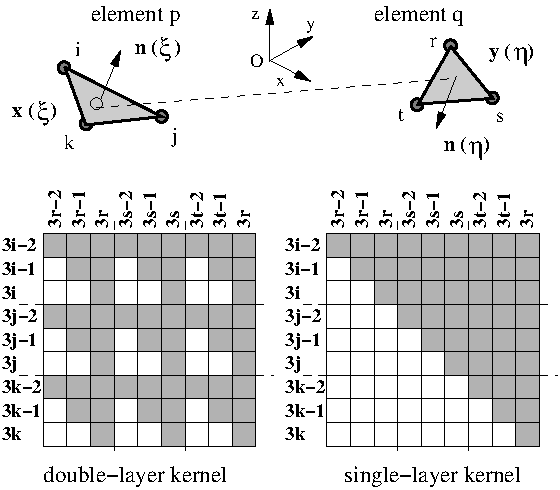
\includegraphics[width=8.6truecm]{./FIG/elemental-simetria-1}
  }% end centerline
}{}% end tema 1
% ..................................................................  
\ifthenelse{\value{tema}=2} {% begin tema 2
  \centerline{%
  \psfig{width=8.6truecm,figure=./FIG/elemental-simetria-1}
  }% end centerline
}{}% end tema 2
%
\caption{%
  The element matrices for the Stokes equation in 3D domains
  using T1 elements \hg {(top)}: (i) double layer kernel 
  ${\tilde{\mathcal{K}}}^{(p,q)}(\bm{x}(\bm{\xi}),\bm{y}(\bm{\eta}))$, %
  symmetric in each 3x3 block (\he{bottom} left); (ii) %
  single-layer kernel 
  ${\tilde{\mathcal{S}}}^{(p,q)}(\bm{x}(\bm{\xi}),\bm{y}(\bm{\eta}))$: %
  symmetric with respect to the main diagonal (\he{bottom} right).}%
\label{fg-elemental-simetria}
\end{figure}
%%%%%%%%%%%%%%%%%%%%%%%%%%%%%%%%%%%%%%%%%%%%%%%%%%%%%%%%%%%%%%%%%%%

% ..................................................................
\subsection{Operation count in the assemblies A0, A1, and A2}
\label{subsubsec:number-operations}

%parrafo
\noindent
The basic element matrix product, given by Eqns.~
(\ref{eq:integral_xi_eta1}-\ref{eq:integral_xi_eta2}), 
defines a standard treatment without any optimization in
the programming of the element matrices. \hg {Therefore,} it 
is not what it should be implemented in a production code.
Nevertheless, it can be chosen as a reference for some
comparisons.
%
Table~\ref{ta:conteo1} contains \hg {the estimates} of the number
of operations (products and sums) by Gauss-Legendre quadrature 
point involved in the evaluation of the A0, A1, and A2 
assemblies, where the count is performed according to the 
coding of the matrix product.
%
However, since the matrix products are performed inside the 
nested double loop $p,q=1,2,...,E$ and inside the quadruple 
loop of numerical quadrature, in practice the percentage 
of reduction will degrade with respect to those indicated 
in Tab.~\ref{ta:conteo1}.
%
It should be noted that for the case of the double-layer kernel 
$\tilde K_{ij}(\bm{x},\bm{y})$, given by Eqn.~(\ref{eq:stokes0110}), 
the reduced assembly A2, given by Eqn.~(\ref{eq:simetria0130}), 
applies. 
%
% ..................................................................
%\ifthenelse{\value{tema}<3}{% begin tema 3
\begin{table*}
  \centering
  \caption{%
    Number of operations (by Gauss-Legendre quadrature point)
    in the assemblies A0, A1, and A2}
  \vspace{2pt}
  \label{ta:conteo1}
  %
  \begin{tabular}{llll}
  \hline  product 
  & A0 [Eqns.~(\ref{eq:simetria0100},\ref{eq:simetria0102})]
  & A1 [Eqns.~(\ref{eq:simetria0100},\ref{eq:simetria0120})]
  & A2 [Eqns.~(\ref{eq:simetria0120},\ref{eq:simetria0130})]\\
  \hline
    %
     &
    $3^2 \times 6 = 54$ &
    $3^2 \times 2 = 18$ &
    $6   \times 2 = 12$ \\
    %
     &
    $3 \times 54 = 162$ &
    not performed       &
    not performed      \\
    %
     &
    $162 + 3^2 \times 54 = 648 $ &
    $      3^2 \times 18 = 162 $ &
    $      3^2 \times 12 = 108 $ \\ 
    %
    relative count \% w.r.t. A0 &
    %\% w.r.t. A0 &
    ---   &
    25~\% &
    17~\% \\
    %
    relative count \% w.r.t. A1 &
    %\% w.r.t. A1 &
    ---   &
    ---   &
    67~\% \\
    %
    \hline
    %
\end{tabular}
\end{table*}
%}{}% end tema 3
% ..................................................................  
%
%
% ++++++++++++++++++++++++++++++++++++++++++++++++++++++++++++++++++
\section{Numerical examples}
\label{sec:numerical-examples}

%parrafo
\noindent
The aim of the examples is to show the time savings
% in applying the strategy
\he {when the assembling algorithm}
which takes advantage of the block symmetries at the
element matrix level \he {is applied}.
%
% Both collocation and Galerkin weighting techniques are applied, 
% where collocation is used as an independent numerical method.
% In the first and second examples, the numerical solutions
% are compared with the analytical ones.
%
In the first and second examples, the wall times for the
three assembling techniques are compared as functions  
of the degrees of freedom number $M$.
%
The remaining examples are introduced to show the benefits
of applying the assembling strategies in problems with
intricate geometries.
%
The numerical solutions computed \hg {with GBEM are validated 
with other numerical methods, as in} \cite{rf:jdelia-gbem2}.
%
%
% The third example is introduced to show the benefits
% of applying the assembling strategies presented in this
% work in problems with intricate geometries.
%
In all \hg {the examples,} a $Q_{22}$ quadrature rule is employed,
where the first subindex denotes the number of Gauss-Legendre (GL)
quadrature points in each surface coordinate used for the
self-integral and for the first layer of neighboring elements,
and the second subindex is the number of GL quadrature points
used for the remaining layers \cite{rf:jdelia-gbem2}. 
%
%
The examples are computed \hg {on %% an E5-1660 
an I7-3930K processor with six cores, using real or complex 
double precision, GFortran compiler, and} main optimization 
flags {\rm -Ofast -march=native -fwhole-file -fwhole-program 
-Warray-temporaries}.  
%
\hy{In all cases, the linear systems are solved with a direct
method through the DGESVX and ZGESVX routines from a LAPACK
library based on the multi-thread ATLAS. These routines also
give the reciprocal of the system matrix condition number
rcond, but at the price of one copy of such matrix}.
%
In the numerical examples LAPACK/ATLAS gives a peak of 
112~GFlops, while the HPL benchmark throws 122~GFlops, 
both in double precision.
%
The LAPACK/ATLAS and HPL software are freely available
at the NETLIB repository (http://www.netlib.org).
%
Also {\rm valgrind} and {\rm gprof} were used in the 
preliminary tests. 
%
Regarding the computation of the system matrix, the $M$ columns
are distributed among the available threads using the OpenMP
directive parallel region, while the {\rm do} loops are executed 
in parallel by the team of threads, where the shared arrays are
synchronized using {\rm critical} and {\rm flush} directives.
%
In order to verify the multi-thread assembly, it was checked
that the linear systems obtained with one or more threads
\hg {are equal to} machine precision.


% ------------------------------------------------------------------
\subsection{Steady Stokes flow around the unit sphere}
\label{subsec:steady-stokes-flow-sphere}

%parrafo
\noindent
This test consists in the steady creeping flow 
around the unit sphere (radius $R=\SI{1}{m}$) 
\cite{rf:tripathi,rf:wang-zhao-wu,rf:lepchev-071202,rf:hewsonrw}.
%
The unperturbed stream has velocity 
$\bm{U}=(1,0,0)\times \SI{10^{-4}}{m/s}$, while 
the dynamic viscosity of the fluid is 
$\mu  = \SI{10^{-3}}{Pa \cdot s}$ and its density is 
$\rho = \SI{1}{kg/m^3}$.
%%
This is a classical test in the literature about
Stokes flow simulation \cite{rf:power-wrobel},
and the numerical results computed with the GBEM
technique, e.g. the traction field on the sphere 
surface, were validated in \cite{rf:jdelia-gbem2}.
%
\hy{The absolute value of the relative error
$|e_r|$ for the Stokes force is computed as
$|e_r|=|F_{\textrm{num}}/F_{\textrm{analytic}}-1|$, with 
$F_{\textrm{analytic}}=F_S$ and $F_S = 6 \pi \mu U R$
is the (steady) Stokes force}.
%
%parrafo
\noindent
\hy {In Fig.}~\ref{fg-simetria-stokes} \hy {the
following magnitudes are plotted as functions of 
the degrees of freedom number $M=3N$:
(i)   the reciprocal of the condition numbers of the
      system matrices rcond (left),
(ii)  the relative errors $|e_r\%|$ in the Stokes
      force (middle left), 
(iii) the wall times required with the assemblies A0-A2 
      and collocation CO (middle right), and
(iv)  the relative wall times between the A1 and A0 assemblies,
      and between the A2 and A1 ones (right)}.
      %
\hg {It can be seen that there is an average reduction in the
wall times of approximately} ${\rstokesone}$~\% \hg {for A1
with respect to A0}, and ${\rstokestwo}$~\% \hg {for A2 with
respect to A1}.
%
%
%%%%%%%%%%%%%%%%%%%%%%%%%%%%%%%%%%%%%%%%%%%%%%%%%%%%%%%%%%%%%%%%%%%
\begin{figure*}[tb]
% ..................................................................
\ifthenelse{\value{tema}=1} {% begin tema 1
  \centerline{%
    \includegraphics[width=16.8truecm,height=5.5truecm]%% =5.4
                    {./FIG/te-galer-q22-stokes-run5}
             }% end centerline
}{}% end tema 1
% ..................................................................
\ifthenelse{\value{tema}=2} {% begin tema 2
  \centerline{%
    \includegraphics[width=16.8truecm,height=5.5truecm]%% =5.4
                    {./FIG/te-galer-q22-stokes-run5}
             }% end centerline
}{}% end tema 2
% ..................................................................
\caption{%
  \hy {Steady Stokes flow. %
  Assemblies A0-A2 and collocation CO, 
  as functions of the degrees of freedom number $M=3N$: 
  (i)   the reciprocal of the condition numbers of the
        system matrices rcond (left),
  (ii)  the relative errors $|e_r\%|$ in the Stokes force
        (middle left), 
  (iii) the wall times required for assemblies A0-A2, and 
        collocation CO (middle right), and 
  (iv)  the relative wall times between the A1 and A0 assemblies,
        and between the A2 and A1 ones (right)}.
  } % end caption
\label{fg-simetria-stokes}
\end{figure*}
%%%%%%%%%%%%%%%%%%%%%%%%%%%%%%%%%%%%%%%%%%%%%%%%%%%%%%%%%%%%%%%%%%%


% ------------------------------------------------------------------
\subsection{Oscillatory Stokes flow around the unit sphere}
\label{subsec:oscillatory-stokes-flow-sphere}

%parrafo
\noindent
This test consists in the oscillatory creeping flow
\cite{rf:wangcy,rf:ishikawa-vladimirov} around the
unit sphere (radius $R=\SI{1}{m}$).
%
\hg{The unperturbed stream has amplitude 
$\bm{U}=(1,0,0)\times \SI{10^{-4}}{m/s}$, 
the dynamic viscosity of the fluid is 
$\mu  = \SI{10^{-3}}{Pa \cdot s}$, its density is 
$\rho = \SI{1}{kg/m^3}$, while the oscillation
frequency is $ f = \SI{10^{-2}}{Hz}$}. 
%
\hy {In this case, the kernel given by Eqn.}
~(\ref{eq:hstokes0110}) \hy {is not symmetric,
although it tends to be symmetric as the frequency
$\Omega \to 0$. Therefore, only the A1 can be applied}.
%
%
\hy{The absolute value of the relative error
$|e_r|$ for the Stokes force is computed as
$|e_r|=|F_{\textrm{num}}/F_{\textrm{analytic}}-1|$, with 
$F_{\textrm{analytic}}=F_S(1 + \zeta + \zeta^2 / 3)$ when the sphere
is at rest and the fluid is oscillating} \cite{rf:pozrikidis2}, 
\hy {where $\zeta=R\sqrt{-I \Omega/\nu}$ and $F_s$ is the steady
Stokes force. In Fig.}~\ref{fg-simetria-oscila} \hy {the
following magnitudes are plotted as functions of the degrees
of freedom number $M=3N$:
(i)   the reciprocal of the condition numbers of the
      system matrices rcond (left),
(ii)  the relative errors $|e_r\%|$ in the Stokes
      force (middle left), 
(iii) the wall times required for the assemblies A0-A1
      (GBEM), and collocation BEM (CO) (middle right), and 
(iv)  the relative wall times between the A0-A1 assemblies
      (right)}.
      %
\hg{As in the previous example, it can be seen that there is
an average reduction in the wall times of approximately:}
${\roscilaone}$~\% \hg {for A1 with respect to A0}.
%
%%%%%%%%%%%%%%%%%%%%%%%%%%%%%%%%%%%%%%%%%%%%%%%%%%%%%%%%%%%%%%%%%%%
\begin{figure*}[t]
% ..................................................................
\ifthenelse{\value{tema}=1} {\centerline{%
    \includegraphics[width=16.8truecm,height=5.5truecm]%% =5.4
                    {./FIG/te-galer-q22-oscila-run5}
}}{}% end tema 1
% ..................................................................
\ifthenelse{\value{tema}=2} {\centerline{%
    \includegraphics[width=16.8truecm,height=5.5truecm]%% =5.4
                    {./FIG/te-galer-q22-oscila-run5}
}}{}% end tema 2
% ..................................................................
\caption{%
  \hy {Oscillatory Stokes flow. %
  Assemblies A0-A1 and collocation CO, 
  as functions of the degrees of freedom number $M=3N$: 
  (i)   the reciprocal of the condition numbers of the
        system matrices rcond (left),
  (ii)  the relative errors $|e_r\%|$ in the Stokes force
        (middle left), 
  (iii) the wall times required for the assemblies A0-A1
        and collocation CO (middle left), and 
  (iv)  the relative wall times between A1 and A0 assemblies
        (right)}.
  }% end caption
  %
\label{fg-simetria-oscila}
\end{figure*}
%%%%%%%%%%%%%%%%%%%%%%%%%%%%%%%%%%%%%%%%%%%%%%%%%%%%%%%%%%%%%%%%%%%


% ++++++++++++++++++++++++++++++++++++++++++++++++++++++++++++++++++
\subsection{Stokes flow around bodies with edges and corners}
\label{subsec:closed-bodies}

%parrafo
\noindent
\hy {Three closed bodies with edges and corners are considered}
\cite{rf:jdelia-gbem2}: \hy {a hollow cube, a sculpted sphere,
and a perforated plate}, each of them immersed
in a creeping flow of a viscous fluid of Newtonian type. 
They are meshed using the NETGEN mesher \cite{rf:netgen}. 
%
\hg {The fluid density is $\rho=1~\mathrm {kg} / \mathrm {m}^3$,
while the kinematic viscosity is $\nu=1~\mathrm{m}^2/\mathrm{s}$.
%
In the first two cases, an uniform steady flow around each body
has incoming velocity of $ U_{\infty}=0.001$ m/s along the $x_1$
direction}.


% ..................................................................
\subsubsection{Hollow cube}
\label{subsec:hollow-cube}

%parrafo
\noindent
The hollow cube (HC) \cite{rf:netgen} is obtained when the 
unit cube is intersected by a sphere and by a complement of 
a sphere, \hg {where the $x_1$ direction coincides with one
of the symmetry axis of the cube}.
%
\hg {The mesh shown in Fig.}~\ref{fg-perforated} \he{(left)}
\hg {has 4~904 nodes and 9~824 elements}.
%
\hy{The wall times required for assembling the system matrix
are given in Table} ~\ref{ta:conteo2} \hy {(left sub-columns)}.


% ..................................................................
\subsubsection{\hy{Sculpted sphere}}
\label{subsec:sculpted-sphere}

%parrafo
\noindent
\hy {The sculpted sphere (SS)} \cite{rf:netgen} \hy {is obtained
when the unit sphere is intersected by a smaller one and by 
three cylinders oriented according to the coordinate axes.
%
The mesh shown in Fig.}~\ref{fg-perforated} \hy {(middle)
has 6~062 nodes and 12~128 elements.
%
When the undisturbed flow is aligned along, for instance, 
the $x_1$ Cartesian axis, the flow is not symmetrical.
%
Furthermore, the mesh is not symmetric.
%
The wall times required for assembling the system matrix are
given in Table} ~\ref{ta:conteo2} \hy {(middle sub-columns)}.

% ..................................................................
%\ifthenelse{\value{tema}<3}{% begin tema 3
\begin{table*}[ht]
  \centering
  \caption{\hy{%
    Wall times (in seconds) and relative times in assembling
    the system matrix for the Stokes flow around: a hollow cube (HC),
    a sculpted sphere (SS), and a perforated plate (PP)}}
  \vspace{2pt}
  \label{ta:conteo2}
  %
  \begin{tabular}{l*{9}r}% equivale a {lrrrrrrrrr}
    \hline
        & \multicolumn{3}{r}%
          {A0, Eqns.~(\ref{eq:simetria0100},\ref{eq:simetria0102})
          \hspace{7mm}} 
        & \multicolumn{3}{r}%
          {A1, Eqns.~(\ref{eq:simetria0100},\ref{eq:simetria0120})
          \hspace{7mm}} 
        & \multicolumn{3}{r}%
          {A2, Eqns.~(\ref{eq:simetria0120},\ref{eq:simetria0130})
          \hspace{7mm}}\\
          %
          & HC & SS & PP & HC & SS & PP & HC & SS & PP \\
          %
    \hline
      wall time for assembly   &
      $436$ & $655$ & $2260$   &
      $237$ & $333$ & $969$    &
      $161$ & $228$ & $713$    \\
    %
      relative time \% w.r.t. A0 &
      ---   &  ---  &  ---       &
      54\%  & 51\%  &  43\%      &
      37\%  & 32\%  &  32\%    \\
    %
      relative time \% w.r.t. A1 &
      ---   &  ---  &  ---       &
      ---   &  ---  &  ---       &
      68\%  &  69\% &  74\%      \\
    %
    \hline
    %
\end{tabular}
\end{table*}
%
%}{}% end tema 3
% ..................................................................

% ..................................................................
\subsubsection{Perforated plate}
\label{subsec:perforated-plate}

%parrafo
\noindent
This is an application case and consists in the oscillatory
Stokes flow around a Perforated Plate (PP) that oscillates
perpendicularly to a fixed substrate \cite{rf:xiao-ye-2011}. 
%%%,rf:ssarraf-enief14}.
%
This case was validated using finite elements
through the PETSc-FEM code \cite{rf:paz3}.
%%
%% ({\it URL}: {\rm http://www.cimec.org.ar/petscfem})
%% This is a parallel multi-physics finite element code
%%
%% rf:garelli-laar2014
%% rf:lbattaglia-jam-06, rf:petscfem-pack,
%% rf:laar041-03-gss, rf:paz3, rf:lbattaglia-ijcfd-10,
%% rf:garibaldi-laar, rf:gfranck-ahmed.
%
It is a 3D intricate geometry which is frequently used in 
MEMS in order to reduce the dissipation of energy due to
the air damping.
%% \cite{rf:magrab-book}.
%
The plate is made of polysilicon and the gap between 
the upper plate and the substrate is $\SI{4}{\micro m}$.
%
The plate dimensions are: 
length $L = L_x = \SI{300}{\micro m}$,
width  $B = L_y = \SI{100}{\micro m}$, and 
height $H = L_z = \SI{  2}{\micro m}$.
%
The height of the substrate is \SI{10}{\micro m}, 
and the plate has 75 equidistant circular holes 
with \SI{4}{\micro m} in radius.
%
The micro-beam is double clamped, at its left end $x=0$
and at its right end $x=L_x$.
%
The maximum amplitude of the harmonic vibration is
$\tilde A=1$ $\mu$m and it is produced at the
center of the micro-beam.  The dynamic viscosity of air
is $\mu=1.86 \times 10^{-11}$ kg/($\mu$m s).
%
\hg {The oscillation frequency is $ f = \SI{17600}{Hz}$}. 
%
The mesh shown in Fig.~\ref{fg-perforated} \hg{(right)}
has 8~697 nodes and 17~686 elements.
%
\hy {The wall times required for assembling the system matrix
in this case, are given in Table} ~\ref{ta:conteo2}
\hy {(right sub-columns)}.
%
%%%%%%%%%%%%%%%%%%%%%%%%%%%%%%%%%%%%%%%%%%%%%%%%%%%%%%%%%%%%%%%%%%%
\begin{figure*}[tb]
% ..................................................................
\ifthenelse{\value{tema}=1} {% begin tema 1
  \centerline{%
   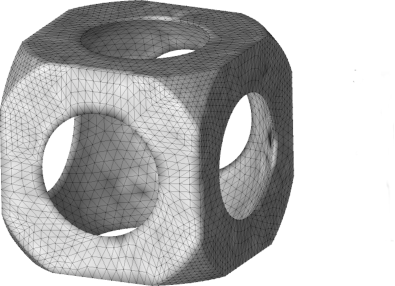
\includegraphics[width=4.6truecm]{./FIG/chueco-9824-b-bw}
   \hspace{0pt}%
   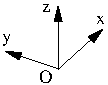
\includegraphics[width=0.8truecm]{./FIG/elemental-simetria-3}
   \hspace{4pt}%   
   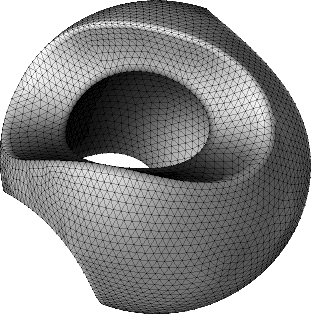
\includegraphics[width=3.4truecm]{./FIG/sculpt-012k}
   \hspace{16pt}%
   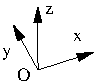
\includegraphics[width=0.8truecm]{./FIG/elemental-simetria-4}
   \hspace{2pt}%   
   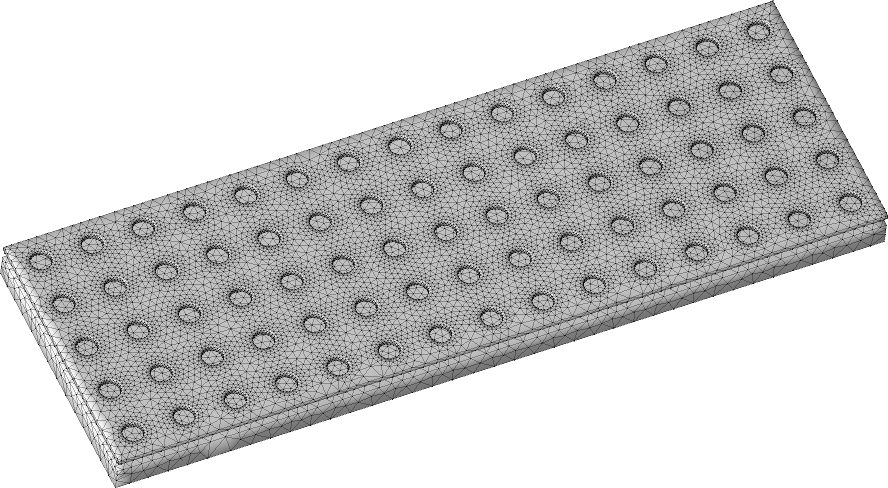
\includegraphics[width=6.2truecm]{./FIG/ra75-17686-dg-ta-bw-2}
             }% end centerline
}{}% end tema 1
% ..................................................................
\ifthenelse{\value{tema}=2} {% begin tema 2
  \centerline{%
  \psfig{width=4.5truecm,figure=./FIG/chueco-9824-b-bw}
  \hspace{6pt}%
  \psfig{width=0.8truecm,figure=./FIG/elemental-simetria-3}
  \hspace{6t}% % triada xyz
  \psfig{width=4.6truecm,figure=./FIG/sculpt-012k}
  \hspace{8pt}%
  \psfig{width=0.8truecm,figure=./FIG/elemental-simetria-4}
  \hspace{6pt}%
  \psfig{width=0.8truecm,figure=./FIG/ra75-17686-dg-ta-bw-2}
           }% end centerline
}{}% end tema 2
% ..................................................................
\caption{%
   \hy {Bodies with edges and corners:
   a hollow cube (HC) (left); 
   a sculpted sphere (SS) (middle); and 
   a perforated plate (PP) (right)} \cite{rf:netgen}.}
\label{fg-perforated}
\end{figure*}
%%%%%%%%%%%%%%%%%%%%%%%%%%%%%%%%%%%%%%%%%%%%%%%%%%%%%%%%%%%%%%%%%%%


% ++++++++++++++++++++++++++++++++++++++++++++++++++++++++++++++++++
\subsection{\hh{Collocation BEM vs. GBEM}} %
\label{sec:performance}

\noindent
\hy {Regarding a comparison between collocation BEM and GBEM, in} 
\cite{rf:jdelia-gbem1} \hy {the folowing properties were stated}
\hh {when they are appplied to BIEs such as the PMH-IF for the
Stokes equation}: \hy{%
(i) in} \hh {GBEM}, \hy {the size of the solution vector is $3N$,
while it is $3E$ in collocation BEM. Since $N \ll E$ for BEM
meshes immersed in 3D domains, then the} \hh{GBEM} \hy {is less
expensive than collocation BEM in core-memory resources,
especially when dense matrices are employed, therefore,
in general, a} \hh {GBEM} \hy {approach allows to use more
refined meshes for a given size of the core memory; (ii)
the system matrix with} \hh {GBEM is symmetric
(only in the steady case)}, \hy {whereas with collocation BEM
it is not; (iii) the net forces obtained with} \hh {GBEM}
\hy {are more accurate than those obtained with collocation
BEM; and (iv)} \hh {GBEM} \hy {exhibits monotonic convergence
while collocation BEM does not.
%
For example, comparisons between GBEM and collocation BEM
applied to the Stokes flow around the unit sphere are shown
in Fig.}~\ref{fg:compa-q22-stokes-run5} \hy {for the steady flow 
using the reduced assemblies A0-A2 and collocation BEM (CO), and
in Fig.}~\ref{fg:compa-q22-oscila-run5} \hy {for the oscillatory
flow using the reduced assemblies A0-A1 and} \hh {CO}.
%%
%% collocation BEM (CO)}.
%%
%%%%%%%%%%%%%%%%%%%%%%%%%%%%%%%%%%%%%%%%%%%%%%%%%%%%%%%%%%%%%%%%%%%
\begin{figure*}[t]
% ..................................................................
\ifthenelse{\value{tema}=1} {\centerline{%
    \includegraphics[width=16.8truecm,height=5.5truecm]%% =5.4
                    {./FIG/te-compa-q22-stokes-run5}
}}{}% end tema 1
% ..................................................................
\ifthenelse{\value{tema}=2} {\centerline{%
    \includegraphics[width=16.8truecm,height=5.5truecm]%% =5.4
                    {./FIG/te-compa-q22-stokes-run5}
}}{}% end tema 2
% ..................................................................
\caption{%
  \hy {Steady Stokes flow. %
  Comparison between GBEM with assemblies A0-A2 and collocation
  CO in the unit sphere and using a $Q_{22}$ quadrature,
  as functions of the degrees of freedom number $M=3N$
  or the number of elements $E$: 
  %
  (i)   the total wall time per Degree Of Freedom (DOF) 
        (left),
  (ii)  the main memory in Mbytes (middle left), 
  (iii) the reciprocal of the condition numbers of the
        system matrix rcond (middle right), and 
  (iv)  the relative errors $|e_r\%|$ in the Stokes
        force (right).}
  }% end caption
  %
\label{fg:compa-q22-stokes-run5}
\end{figure*}
%%%%%%%%%%%%%%%%%%%%%%%%%%%%%%%%%%%%%%%%%%%%%%%%%%%%%%%%%%%%%%%%%%%
%
%%%%%%%%%%%%%%%%%%%%%%%%%%%%%%%%%%%%%%%%%%%%%%%%%%%%%%%%%%%%%%%%%%%
\begin{figure*}[t]
% ..................................................................
\ifthenelse{\value{tema}=1} {\centerline{%
    \includegraphics[width=16.8truecm,height=5.5truecm]%% =5.4
                    {./FIG/te-compa-q22-oscila-run5}
}}{}% end tema 1
% ..................................................................
\ifthenelse{\value{tema}=2} {\centerline{%
    \includegraphics[width=16.8truecm,height=5.5truecm]%% =5.4
                    {./FIG/te-compa-q22-oscila-run5}
}}{}% end tema 2
% ..................................................................
\caption{%
  \hy {Oscillatory Stokes flow. %
  Comparison between GBEM with assemblies A0-A1 and collocation
  BEM (CO) in the unit sphere and using a $Q_{22}$ quadrature,
  as functions of the degrees of freedom number $M=3N$
  or the number of elements $E$: 
  %
  (i)   the total wall time per Degree Of Freedom (DOF) 
        (left),
  (ii)  the main memory in Mbytes (middle left), 
  (iii) the reciprocal of the condition numbers of the
        system matrix rcond (middle right), and 
  (iv)  the relative errors $|e_r\%|$ in the Stokes
        force (right).}
  }% end caption
  %
\label{fg:compa-q22-oscila-run5}
\end{figure*}
%%%%%%%%%%%%%%%%%%%%%%%%%%%%%%%%%%%%%%%%%%%%%%%%%%%%%%%%%%%%%%%%%%%

% ------------------------------------------------------------------
%parrafo
\noindent
\he {Regarding the relative error of the Stokes force versus 
the total wall time, defined as the sum of the wall time
consumed by the matrix assembly plus the solution of the
linear system, e.g. through an Lower-Upper (LU) factorization,
in Fig.}~\ref{fg-error-walltime}, \he {the relative error $|e_r\%|$
of the Stokes force in the unit sphere case is plotted as a function 
of the total wall time, and using GBEM with assemblies A0-A2 and 
collocation BEM (CO) in the steady creeping flow (left) and 
oscillatory one (right), where it can be seen that there is a 
crossing between the GBEM and collocation BEM curves, i.e. 
GBEM is cheaper than collocation BEM for more refined meshes}.
%
%%%%%%%%%%%%%%%%%%%%%%%%%%%%%%%%%%%%%%%%%%%%%%%%%%%%%%%%%%%%%%%%%%%
\begin{figure}[ht]
% ..................................................................
\ifthenelse{\value{tema}=1} {% begin tema 1
  \centerline{%
    \includegraphics[width=8.4truecm,height=5.5truecm]%% =5.4
                    {./FIG/te-galdi-q22-stokes-run5}
             }% end centerline
}{}% end tema 1
% ..................................................................
\ifthenelse{\value{tema}=2} {% begin tema 2
  \centerline{%
    \includegraphics[width=8.4truecm,height=5.5truecm]%% =5.4
                    {fig9}
             }% end centerline
}{}% end tema 2
% ..................................................................
\caption{\he{%
  Relative error $|e_r\%|$ of the Stokes force in the unit 
  sphere case as a function of the total wall time, and using 
  GBEM with assemblies A0-A2 and collocation BEM (CO): 
  (i)  steady creeping flow (left), and 
  (ii) oscillatory one (right).}} % end caption
\label{fg-error-walltime}
\end{figure}
%%%%%%%%%%%%%%%%%%%%%%%%%%%%%%%%%%%%%%%%%%%%%%%%%%%%%%%%%%%%%%%%%%%


% ++++++++++++++++++++++++++++++++++++++++++++++++++++++++++++++++++
\section{Conclusions}
\label{sec:conclusions}

% parrafo
\noindent
The harnessing of symmetries in the element interaction 
integrals in Galerkin BEM can be introduced into a standard 
implementation through minor changes at the element level.
%
\hg {According to the test cases solved in this work,
it can be concluded that a meaningful reduction in the wall
time needed for assembling the system matrix can be reached
using the reduced assembly strategy A2.
On average, it is found to be $\rstokestwo$\% faster than the
A1 procedure}.
%%
\hy{The reduced assembly A2 %% presented in this work
is based on block symmetries at the element level which are
due to symmetries of the kernels and do not depend on those
of the flow nor of the mesh.}
%
%% According to the tests solved, it can be concluded that a 
%% meaningful reduction in the wall time needed for assembling
%% the system matrix can be reached using on average of
%% $\rstokestwo$\% with respect to the A1 case using the
%% reduced assembly A2, \hg {which is based on block symmetries
%% at the element level due to symmetries of the kernels and not
%% those of the flow nor in the mesh}. 
%
The examples with intricate geometries allow to conclude 
that the reduction in the computation time for the assembly 
process is \hg{almost} independent of the mesh details.

% ++++++++++++++++++++++++++++++++++++++++++++++++++++++++++++++++++
%% Chequear proyectos 
%% \acks                   % IJNME
%% \begin{acknowledgment}  % ASME


\noindent
\ltitle{Acknowledgments}
%\smallskip
%%
\noindent
This work has received financial support from
%
% Consejo Nacional de Investigaciones Cient\'{\i}ficas y 
% T\'ecnicas (CONICET, Argentina, grant %
%
CONICET (Argentina, grants %
PIP 112-20111-978), %      % --> 2013-2015 mstorti
%
% Universidad Nacional del Litoral (UNL, Argentina, grant %
UNL (Argentina, grant %
%CAI+D 2009--III-4--2), %    % --> 2009-2011 jdelia
 CAI+D 2011-01-00134-LI, and % --> 2014-2017 vsonzogni
 CAI+D 2011-01-00012-LI), %  % --> 2013-2016 grios
%
% Agencia Nacional de Promoci\'on Cient\'{\i}fica y 
% Tecnol\'ogica (ANPCyT, Argentina, grants
ANPCyT (Argentina, grants %
%PICT-2006-1506,            % --> 2008-2011 vsonzogni
%PICT-2007-1141,            % --> 2009-2011 mstorti
%PAE-2004-22592-nodo-22961  % --> 2009-2011 acardona
%PICT-2010-2492,            % --> 2010-2013 jdelia
%PICT-PRH-2009-0147,        % --> 2012-2014 elopez
 PICT-2014-2660, %          % --> 2010-2013 jdelia
 PICT-E-2014-0191, and %    % --> 2014-2014 jdelia
 PICT-2013-0938), %         % --> 2015-2016 lbattaglia
%
% the European Commission under the 7th framework program, 
% Marie-Courie actions, people, International Research Staff 
% Exchange Scheme (grant ''Numerical simulation in technical 
% sciences'', NumSim PIRSES-GA2009-246977),
%
% Universidad Nacional del Comahue (UNCo, Argentina,
UNCo (Argentina, grant 04/I-215), %
%
and was performed with the %
{\rm Free Software Foundation/GNU-Project} resources as
% GNU--Linux~OS, GNU--GFortran, GNU--Octave, GNU--GIMP,
Linux~OS and GFortran, %% Octave, GIMP,
as well as other Open Source resources such as 
NETGEN and OpenDX. %%, %% {ParaView}, {Xfig}, and \LaTeX{}.

%%%%%%%%%%%%%%%%%%%%%%%%%%%%%%%%%%%%%%%%%%%%%%%%%%%%%%%%%%%%%%%%%%%%%%
% The bibliography is stored in an external database file
% in the BibTeX format (file_name.bib).  The bibliography is
% created by the following command and it will appear in this
% position in the document. You may, of course, create your
% own bibliography by using thebibliography environment as in
%
% \begin{thebibliography}{12}
% ...
% \bibitem{itemreference} D. E. Knudsen.
% {\em 1966 World Bnus Almanac.}
% {Permafrost Press, Novosibirsk.}
% ...
% \end{thebibliography}
%
% Here's where you specify the bibliography style file.
% The full file name for the bibliography style file 
% used for an ASME paper is asmems4.bst.
\bibliographystyle{asmems4}

% Here's where you specify the bibliography database file.
% The full file name of the bibliography database for this
% article is asme2e.bib. The name for your database is up
% to you.
\bibliography{navales}



% ++++++++++++++++++++++++++++++++++++++++++++++++++++++++++++++++++++
%% % Avoid Appendices if possible...
\appendix       %%% starting appendix

% %%%%%%%%%%%%%%%%%%%%%%%%%%%%%%%%%%%%%%%%%%%%%%%%%%%%%%%%%%%%%%%%%%
\begin{table}[tb]
  \centering
  \caption{\hy {Integration coordinates $\bm {\mu}_n, \bm {\xi}_n$
    and Jacobian $J_n$, as a function of the coordinates
    $0 \le  \omega, x, \chi_1, \chi_2 \le 1$ in  the case
    of the self--integrals $\bm {I_1}-\bm {I}_3$}  
    \cite{rf:taylordj1,rf:jdelia-gbem1}}
  \smallskip
  \label{ta:duffy_panel_comun2}
  \begin{tabular}{llll}
    \hline\noalign{\smallskip}
                 &
   $ \bm {I}_1 $ &
   $ \bm {I}_2 $ &
   $ \bm {I}_3 $ \\
    \noalign{\smallskip}\hline\noalign{\smallskip}
 % F1
 $ \mu_1    $  &
 $ \omega   $  &
 $ \omega x $  &
 $ \omega x $  \\
 %
 % F2
 $ \mu_2    $      &
 $ \omega x $      &
 $ \omega (x - 1)$ &
 $ \omega        $ \\
 % F3
 $ \xi_{1}                                     $ &
 $ (1 - \mu_1)         \chi_1                  $ &
 $ (1 - \mu_1 + \mu_2) \chi_1 - \mu_2          $ &
 $ (1 - \mu_2) \chi_1  $ \\ %% + \mu_2 - \mu_1 
 %
 % F3b
 $                                             $ &
 $                                             $ &
 $                                             $ &
 $ + (\mu_2 - \mu_1)                            $ \\
 % F4
 $ \xi_{2}                                     $ &
 $ \xi_1 \chi_2                                $ &
 $ (\xi_1 + \mu_2) \chi_2 - \mu_2              $ &
 $ (\xi_1 - \mu_2 + \mu_1) \chi_2              $ \\
 %
 % F5
 $ J_n                                         $ &
 $ (1 - \mu_1)          \xi_1                  $ &
 $ (1 - \mu_1 + \mu_2) (\xi_1 + \mu_2)          $ &
 $ (1 - \mu_2) (\xi_1 - \mu_2 + \mu_1) $ \\
 %
 % F5b
 %$                                             $ &
 %$                                             $ &
 %$                                             $ &
 %$ \times (\xi_1 - \mu_2 + \mu_1) $ \\
\noalign{\smallskip}\hline
\end{tabular}
\end{table}
% %%%%%%%%%%%%%%%%%%%%%%%%%%%%%%%%%%%%%%%%%%%%%%%%%%%%%%%%%%%%%%%%%%


% ++++++++++++++++++++++++++++++++++++++++++++++++++++++++++++++++++
\section*{\hy{Appendix A: The extended Taylor scheme}} %
\label{rf:appendix-a}

\noindent
\hy {Without loss of generality, Eqns.} 
(\ref{eq:integral_xi_eta_todo1}-\ref{eq:integral_xi_eta_todo2}) 
\hy {can be written as}
%
\begin{equation}
  \bm {I} =
     \int_{0}^{1}     \dif \xi_1 ~
     \int_{0}^{\xi_1}  \dif \xi_2 ~
     \int_{0}^{1}     \dif \eta_1 ~
     \int_{0}^{\eta_1} \dif \eta_2 ~
     \bm {f} (\bm {\xi},\bm {\eta})
\label{eq:integral_xi_eta}
\end{equation}
%
\hy {The Taylor strategy to evaluate Eqn.} (\ref{eq:integral_xi_eta})
\hy {is designed specifically for flat simple triangles $p$ and $q$
when they are contiguous or coincidents, and the integrand
$\bm {f} (\bm {\xi}, \bm {\eta})$ has a weak singularity.
In that case, the relative coordinates} 
$ \mu_1 = \eta_1 - \xi_1 $ and $\mu_2 = \eta_2 - \xi_2$
%
%% \begin{equation}
%%   \begin{aligned}
%%    \mu_1 & = \eta_1 - \xi_1  \cr
%%    \mu_2 & = \eta_2 - \xi_2
%%   \end{aligned}
%% \label{eq:coordenadas_relativas}
%% \end{equation}
%
\hy {are introduced. The replacement of these coordinates 
into Eqn.} (\ref{eq:integral_xi_eta}) \hg {leads to}
%
\begin{equation}
  \bm {I} =
      \int_0^1                       \di \xi_1
      \int_{-\xi_1}^{1-\xi_1}          \di \mu_1
      \int_0^{\xi_1}                  \di \xi_2
      \int_{-\xi_2}^{\mu_1+\xi_1-\xi_2} \di \mu_2 ~
      \bm {f} (\bm {\xi},\bm {\mu})
\label{eq:integral_xi_mu}
\end{equation}
%
\hy {Changing the integration order $(\mu_2,\xi_2,\mu_1,\xi_1)$ 
to the order $(\xi_2,\xi_1,\mu_2,\mu_1)$, combining integrals 
that have overlapping domains, and introducing several Duffy
coordinate transformations, Eqn.}~(\ref {eq:integral_xi_eta})
\hy {is split into 3, 6 and 1 independent integrals for the 
common facets, common edge, and common vertex cases, 
respectively.
%
It should be noted that the new integration order 
moves the weak singularity to the origin, the overlapping 
domains occur in the plane of the relative coordinates
$(\mu_1, \mu_2)$, while the Duffy coordinate transformations
regularize the integrands by using polar coordinates, 
and the selected ones are the same used by Taylor.
%
In principle, there are 6 independent integrals in
each case, although, with further considerations in
the common facet and common vertex cases, they are
reduced to 3 and 1, respectively.
%
The final expressions are given in the next sections, 
where the following notations are used:}
$\tilde{\bm{f}_n}=\tilde{\bm{f}}(\bm{\xi}_n,\bm{\eta}_n)$, 
where $\tilde{\bm{f}}(\bm{\xi}_n,\bm{\eta}_n)=$%
$\bm{f}(\bm{\xi}_n,\bm{\eta}_n)+\bm{f}(\bm{\eta}_n,\bm{\xi}_n)$,
and $\bm {\eta}_n = \bm {\xi}_n + \bm {\mu}_n $.
%% , while for $\bm {\xi}_n, \bm {\mu}_n$  see each case.
%
%% \begin{equation}
%%   \begin{aligned}
%%     \tilde {\bm {f}_n} & =
%%     \tilde {\bm {f}}(\bm {\xi}_n,\bm {\eta}_n) =
%%       \bm {f} (\bm {\xi}_n,\bm {\eta}_n) 
%%     + \bm {f}(\bm {\eta}_n,\bm {\xi}_n) \cr
%%     \bm {\eta}_n & = \bm {\xi}_n 
%%     + \bm {\mu}_n \cr
%%     \bm {\xi}_n, & ~ \bm {\mu}_n ~ : ~ \textrm {see each case}
%%   \end{aligned}
%% \label{eq:gbemvar0}
%% \end{equation}

% %%%%%%%%%%%%%%%%%%%%%%%%%%%%%%%%%%%%%%%%%%%%%%%%%%%%%%%%%%%%%%%%%%
\begin{table}[tb]
  \centering
  \caption{\hy {
      Integration coordinates $\bm {\mu}_n$ and $\bm {\xi}_n$,
      as a function of the coordinates
      $0 \le  \omega, x_1, x_2, \chi_1 \le 1$ in
      the integrals with a common edge $\bm {I}_4-\bm {I}_9$}
    \cite{rf:taylordj1,rf:jdelia-gbem1}}
  \smallskip
  \label{ta:duffy_arista_comun2}
  \begin{tabular}{lllll}
    \hline\noalign{\smallskip}
   $n$ & %% $ \bm {I}_n $
   $ \mu_1$        &
   $ \mu_2 $       &
   $ \xi_1$        &
   $ \xi_2$        \\
  \noalign{\smallskip}\hline\noalign{\smallskip}
 $ 4 $                    &
 $ -\omega x_1 $                  &
 $ -\omega x_1 x_2$               &
 $ (1 - \omega) \chi_1 + \omega $ &
 $ \omega (1 - x_1 + x_1 x_2) $   \\
 %
 $ 5 $                    &
 $ \omega x_1 $                   &
 $ \omega x_1 x_2$                &
 $ (1-\omega) \chi_1 $            &    %% $ + \omega (1 - x_1) $ 
 $ \omega (1 - x_1)               $ \\
 %
                                  &
                                  &
                                  &
 $ + \omega (1 - x_1) $           &
                                    \\
 %
 $ 6 $                    &
 $ -\omega x_1 x_2$               &
 $  \omega x_1 (1 - x_2) $        &
 $ (1 - \omega) \chi_1 + \omega $ &
 $ \omega (1 - x_1)             $ \\
 %
 $ 7 $                    &
 $ \omega x_1 x_2       $         &
 $ \omega x_1 (x_2 - 1) $         &
 $ (1 - \omega) \chi_1  $         &  %% $ + \omega (1 - x_1 x_2) $
 $ \omega (1 - x_1 x_2)         $ \\
 %
                                  &
                                  &
                                  &
 $ + \omega (1 - x_1 x_2) $       &
                                  \\
 %
 $ 8 $                    &
 $ -\omega x_1 x_2 $              &
 $ -\omega x_1 $                  &
 $ (1 - \omega) \chi_1 + \omega $ &
 $ \omega                       $ \\
 %
 $ 9 $                    &
 $  \omega x_1 x_2 $              &
 $  \omega x_1 $                  &
 $ (1 - \omega) \chi_1 $          & %% $+ \omega (1 - x_1 x_2) $
 $ \omega (1 - x_1)               $ \\
 %
                                  &
                                  &
                                  &
 $ + \omega (1 - x_1 x_2) $       &
 $ \omega (1 - x_1) $             \\
  \noalign{\smallskip}\hline
\end{tabular}
\end{table}
% %%%%%%%%%%%%%%%%%%%%%%%%%%%%%%%%%%%%%%%%%%%%%%%%%%%%%%%%%%%%%%%%%%


% ++++++++++++++++++++++++++++++++++++++++++++++++++++++++++++++++++
\subsubsection*{\hy{Common facets}}

\noindent
\hy {In the case of flat common facets, Taylor found that the
symmetry reduces the number of integrals from six to three,
given by Eqn.}~(\ref {eq:commonfacets})
%
\begin{equation}
  \bm {I} = \sum_{n=1}^3 \bm {I}_n 
  \quad \textrm {with} \quad
  \bm {I}_n  =  \int_{0}^{1}  \di \omega
                \int_{0}^{1}  \di x
                \int_{0}^{1}  \di \chi_1
                \int_{0}^{1}  \di \chi_2 ~
             ~ \tilde {J_n} ~ \tilde {\bm{f}_n}
\label{eq:commonfacets} 
\end{equation}
%
\hy{%
where $(\omega$, $x$, $\chi_1$, $\chi_2)$ are the GL quadrature points,
while $\bm {\xi}_n=\bm{\xi}_n(\omega,x,\chi_1,\chi_2)=(\xi_1,\xi_2)_n$,
and 
$\bm {\mu}_n=\bm{\mu}_n(\omega,x,\chi_1,\chi_2)=(\mu_1,\mu_2)_n$,
where the intervals $ 0 \le \omega, x, \chi_1, \chi_2 \le 1 $ 
are the usual unit interval for the GL quadrature points.
%
The coordinates $\bm {\mu}_n$ and $\bm {\xi}_n$ are computed 
using rows 1-2 and 3-4 of Table} \ref{ta:duffy_panel_comun2},
\hy {respectively, and the Jacobian is obtained as
%% $ {\tilde J}_n = J_a J_n $, with $J_a=\omega$,
%% while $J_n$ is given in the row 5 of Table}
$ {\tilde J}_n = \omega J_n $, while $J_n$ is
given in the row 5 of Table} \ref{ta:duffy_panel_comun2}.

% ++++++++++++++++++++++++++++++++++++++++++++++++++++++++++++++++++
\subsubsection*{\hy{Common edge}}

\noindent
\hy {In the case of a common edge, six integrals must be computed, 
and given by Eqn.}~(\ref{eq:commonedge-10})
%
\begin{equation}
    \bm {I} = \sum_{n=4}^9 \bm {I}_n 
    \quad \textrm {with} \quad
    \bm {I}_n =  \int_{0}^{1}  \di \omega
                  \int_{0}^{1}  \di x_1
                  \int_{0}^{1}  \di x_2
                  \int_{0}^{1}  \di \chi_1 ~
                ~ \tilde {J_n} ~ \tilde {\bm{f}_n}
\label{eq:commonedge-10}
\end{equation}
%
\hy {where the intervals
$ 0 \le \omega, x_1, x_2, \chi_1 \le 1 $ are
the usual unity interval for the GL quadrature points.
%
The coordinates $\bm {\mu}_n$ and $\bm {\xi}_n$ are computed using
columns 1-2 and 3-4 of Table} \ref{ta:duffy_arista_comun2},
\hy {respectively, and the Jacobian is obtained as
$ {\tilde J}_n = (1 - \omega) x_1 \omega^2 $}.
%%
%% $ {\tilde J}_n = J_b \overline {J} $, with $J_b= x_1 \omega^2$
%% and $\overline {J} = 1 - \omega$}.

% ++++++++++++++++++++++++++++++++++++++++++++++++++++++++++++++++++
\subsubsection*{\hy{Common vertex}}

\noindent
\hy {Finally, in the case of a common vertex, the six integrals 
are reduced to one, and given by Eqn.}~(\ref{eq:common-vertex})
%
\begin{equation}
   \bm {I}_{10} = \int_{0}^{1}  \di \omega
                 \int_{0}^{1}  \di z_1
                 \int_{0}^{1}  \di z_2
                 \int_{0}^{1}  \di z_3 ~
                ~ \tilde {J_{10}} ~ \tilde {\bm{f}_{10}}
\label{eq:common-vertex}
\end{equation}
%
\hy {where the intervals $ 0 \le \omega, z_1, z_2, z_3 \le 1 $ are
the usual unity interval for the GL quadrature points.
%
The coordinates $\bm {\xi}_{10}$ and $\bm {\eta}_{10}$ are computed 
using columns 1-2 and 3-4 of Table} \ref{ta:duffy_vertex_comun2},
\hy {respectively, and the Jacobian is obtained as
   $ {\tilde J}_{10} = z_2 \omega^3$.}
%% $ {\tilde J}_{10} = J_c $, with $J_c = z_2 \omega^3$.}

% %%%%%%%%%%%%%%%%%%%%%%%%%%%%%%%%%%%%%%%%%%%%%%%%%%%%%%%%%%%%%%%%%%
\begin{table}[tb]
  \centering
  \caption{ \hy {%
      Integration coordinates $\bm {\xi}_{10}$ and $\bm {\eta}_{10}$,
      as a function of the coordinates
      $0 \le \omega, z_1, z_2, z_3 \le 1$ in
      the integral with a common vertex $\bm {I}_{10}$}
      \cite{rf:taylordj1,rf:jdelia-gbem1}}
  \smallskip
  \label{ta:duffy_vertex_comun2}
  \begin{tabular}{lllll}
    \hline\noalign{\smallskip}
                    &
   $  \xi_1 $       &
   $  \xi_2 $       &
   $ \eta_1 $       &
   $ \eta_2 $       \\
  \noalign{\smallskip}\hline\noalign{\smallskip}
 $  \bm {I}_{10}   $  &
 $  \omega         $  &
 $  \omega z_1     $  &
 $  \omega z_2     $  &
 $  \omega z_2 z_3 $ \\
  \noalign{\smallskip}\hline
\end{tabular}
\end{table}
% %%%%%%%%%%%%%%%%%%%%%%%%%%%%%%%%%%%%%%%%%%%%%%%%%%%%%%%%%%%%%%%%%%

% ++++++++++++++++++++++++++++++++++++++++++++++++++++++++++++++++++
\section*{\hy{Appendix B: a BIE with a scalar kernel}} %
\label{rf:appendix-b}

\noindent
\hy {In order to show the application of the proposed assembling
algorithm to others cases aside from the Stokes flow, this
appendix includes results for a BIE with a scalar kernel}.

% ..................................................................
\subsection*{\hy{Reduced assembly A3}}
\label{subsubsec:assembly-a3}

%parrafo
\noindent
\hy{The reduced assembly A2 cannot be applied to BIEs with scalar
kernels like those related to the Laplace or Helmholtz equations.
%
Nevertheless, other symmetries can be taken into account.
For instance, in} \cite{rf:gray-griffith} \hy {it is taken into
account that the matrices of interaction between any pair of
elements $p-q$ share the same geometric quantities except, in
general, the unit normals $\bm {n} (\bm {x})$ and
$\bm {n} (\bm {y})$, therefore it is convenient to compute
both matrices simultaneously. This kind of strategy defines the
reduced assembly A3 that can be used in BIEs with a scalar kernel,
as the Morino Integral Formulation} \cite{rf:morino}
\hy{(or Morino-IF for short)}. 
  
% ..................................................................
\subsection*{\hy{The Morino integral formulation}}
\label{subsec:morino-if}

% parrafo
\noindent
\hy{The Morino-IF consists in a BIE for the exterior Neumann
problem of the Laplace equation over a rigid, closed, piecewise
smooth surface $A$ in $\mathbb{R}^3$} \cite{rf:morino}
\hy{that can be written as} 
%
\begin{equation}
  \frac {1} {2} \lambda (\bm {x}) - \int_A
  \tilde D (\bm {x}, \bm {y}) \lambda (\bm {y}) \dif A_{\bm {y}}
  =
  \int_A \tilde C (\bm {x}, \bm {y}) ~
  \sigma (\bm {x}) \dif A_{\bm {y}}
  %
\label{eq:morino0100}
\end{equation}
%
\hy{for all $\bm{x} \in A$, where $\lambda (\bm {x})$ is 
the double-layer surface density, and $\sigma (\bm {x})$ 
is the single-layer surface density.
%
The single-layer $\tilde C (\bm {x},\bm {y})$ and 
the double-layer $\tilde D(\bm{x},\bm{y})$ kernels 
for the Laplace equation are given by 
$ \tilde C (\bm {x},\bm {y}) =  \hat{c}/r$, and  
$ \tilde D (\bm {x},\bm {y}) = -\hat{c} r_k n_k (\bm{y})/r^3 $,
where $\hat{c}=1/(4 \pi)$}.
%
% ..................................................................
%% \ifthenelse{\value{tema}<3}{% begin tema 3
%%   \begin{subequations}
%%   \begin{align}
%%     %
%%     \tilde C (\bm {x},\bm {y}) & = \frac {1} {4 \pi}
%%                                    \frac {1} {r} 
%%     \label{eq:morino0120} \\
%%     %
%%     \tilde D (\bm{x},\bm{y}) & = - \frac {1} {4 \pi}
%%     \frac {r_k} {r^3} n_k (\bm{y})
%%     %
%%     \label{eq:morino0130}
%%      %
%%   \end{align}
%%   \end{subequations}
%% %
%% }{}% end tema 3
% ..................................................................
%
\hy{In addition, $\sigma(\bm{x})=-U_k(\bm{x})n_k(\bm{x})$ is the 
value needed to cancel the component of the velocity in the
normal direction to the surface $A$.
%
In this way, the right hand side of Eq.}~(\ref{eq:morino0100})
\hy{is given and, hence, the Morino-IF is reduced to a 
Fredholm BIE of second kind with weakly singular kernels 
for $\lambda(\bm{x})$}.
%
%
%%%%%%%%%%%%%%%%%%%%%%%%%%%%%%%%%%%%%%%%%%%%%%%%%%%%%%%%%%%%%%%%%%%
\begin{figure*}[tb]
% ..................................................................
\ifthenelse{\value{tema}=1} {% begin tema 1
  \centerline{%
    \includegraphics[width=16.8truecm,height=5.5truecm]%% =5.4
                    {./FIG/te-galer-q22-morino-run5}
             }% end centerline
}{}% end tema 1
% ..................................................................
\ifthenelse{\value{tema}=2} {% begin tema 2
  \centerline{%
    \includegraphics[width=16.8truecm,height=5.5truecm]%% =5.4
                    {./FIG/te-galer-q22-morino-run5}
             }% end centerline
}{}% end tema 2
% ..................................................................
\caption{%
  \hy {Rankine closed body. %
  Assemblies A0, A1, A3 and collocation CO, 
  as functions of the degrees of freedom number $M=N$: 
  (i)   the reciprocal of the condition numbers of the
        system matrix rcond (left),
  (ii)  the Mean Squared Error $\textrm {MSE}\%$ in the
        dipolar density $\lambda$ (middle left), 
  (iii) the wall times required for assemblies A0, A1, A3, and 
        collocation CO (middle right), and 
  (iv)  the relative wall times between the A1 and A0 assemblies,
        and between the A3 and A1 ones (right)}.
  } % end caption
\label{fg-simetria-morino}
\end{figure*}
%%%%%%%%%%%%%%%%%%%%%%%%%%%%%%%%%%%%%%%%%%%%%%%%%%%%%%%%%%%%%%%%%%%
%
% ..................................................................
%
% ..................................................................
\subsubsection*{\hy{Galerkin weighting technique for the Morino-IF}}
\label{subsec:galerkin-laplace-peso}

% parrafo
\noindent
\hy{The application of the Galerkin weighting to} Eq.
(\ref{eq:morino0100}), \hy{using T1 elements and after algebraic
handling, leads to the linear equation system} %%% (LES)
%
\begin{equation}
    \sum_{p=1}^E \sum_{q=1}^E \left  [
    \frac {1} {6} A^{(p)} \delta^{(p,q)} \bm {I}_3 -  
    \mathcal {L}^{(p,q)} \right ] \bm {\lambda}^{(q)} =
    %
    \sum_{p=1}^E \sum_{q=1}^E
    \mathcal {Q}^{(p,q)} \bm {\sigma}^{(q)}
\label{eq:morino0300}
\end{equation}
%
\hy {where $\delta^{(p,q)}$ is the Kronecker delta,
$\bm {I}_3 $ is the $3 \times 3$ identity matrix, and}
%% the following notation is employed
%
\begin{equation}
  \mathcal {L}^{(p,q)} =
  \int_{A^{(p)}}  \dif A_{\bm {x}}
  \int_{A^{(q)}}  \dif A_{\bm {y}} \left  [
  \bm {N}^{(p)T} (\bm {x}) ~ \tilde {D} (\bm {x},\bm {y}) ~
  \bm {N}^{(p)}  (\bm {x}) \right  ]
\label{eq:morino0310}
\end{equation}
%
\hy {is the elemental matrix of the system, while
the corresponding elemental matrix for the load term
is given by}
%
\begin{equation}
  \mathcal {Q}^{(p,q)} =
  \int_{A^{(p)}}  \dif A_{\bm {x}}
  \int_{A^{(q)}}  \dif A_{\bm {y}} \left  [
  \bm {N}^{(p)T} (\bm {x}) ~ \tilde {C} (\bm {x},\bm {y}) ~
  \bm {N}^{(q)}  (\bm {y}) \right  ]
\label{eq:morino0320}
\end{equation}
%
\hy {The elemental vectors for the solution and the right
hand side of Eq.} (\ref{eq:morino0300}) are
%
\begin{equation}
  \bm {\lambda}^{(q)} =
  \begin{bmatrix} \lambda_r \cr \lambda_s \cr \lambda_t \end{bmatrix}
  %% \in \mathbb{R}^{3 \times 1}
  \qquad \textrm {and} \qquad
  \bm {\sigma}^{(q)} =
  \begin{bmatrix} \sigma_r \cr \sigma_s \cr \sigma_t \end{bmatrix}
  %% \in \mathbb{R}^{3 \times 1}
\label{eq:morino0330}
\end{equation}
%
\hy{respectively. In this case, the interaction matrix of $p$
 element (nodes $i,j,k$) with a $q$ element (nodes $r,s,t$), see
Fig.}~\ref{fg-notation-gbem} \hy{(left), has the form} 
%
% ..................................................................
\begin{equation}
    \underset {\scriptscriptstyle 3 \times 3}
    {{\mathcal{L}}^{(p,q)}} = 
    %
    \begin{bmatrix}
      %
         {\mathcal {L}}^{(p,q)}_{i,r}  &
         {\mathcal {L}}^{(p,q)}_{i,s}  &
         {\mathcal {L}}^{(p,q)}_{i,t}  \cr
      %
         {\mathcal {L}}^{(p,q)}_{j,r}  &
         {\mathcal {L}}^{(p,q)}_{j,s}  &
         {\mathcal {L}}^{(p,q)}_{j,t}  \cr
      %
         {\mathcal {L}}^{(p,q)}_{k,r}  &
         {\mathcal {L}}^{(p,q)}_{k,s}  &
         {\mathcal {L}}^{(p,q)}_{k,t} 
      %
    \end{bmatrix}
    \label{eq:gray0100}
\end{equation}
% ..................................................................
%
\hy{and the elemental interaction matrix of the $q$ element
with the $p$ element, has the form}
%
% ..................................................................
\begin{equation}
    \underset {\scriptscriptstyle 3 \times 3}
    {{\mathcal {L}}^{(q,p)}} = 
    %
    \begin{bmatrix}
      %
         {\mathcal {L}}^{(q,p)}_{r,i}  &
         {\mathcal {L}}^{(q,p)}_{r,j}  &
         {\mathcal {L}}^{(q,p)}_{r,k}  \cr
      %
         {\mathcal {L}}^{(q,p)}_{s,i}  &
         {\mathcal {L}}^{(q,p)}_{s,j}  &
         {\mathcal {L}}^{(q,p)}_{s,k}  \cr
      %
         {\mathcal {L}}^{(q,p)}_{t,i}  &
         {\mathcal {L}}^{(q,p)}_{t,j}  &
         {\mathcal {L}}^{(q,p)}_{t,k} 
      %
    \end{bmatrix}
    \label{eq:gray0110}
\end{equation}
% ..................................................................
%
\hy{Equations}~(\ref{eq:gray0100}-\ref{eq:gray0110})
\hy{involves many common geometric operations except the
unit normals $\bm {n} (\bm {x})$ (on the $p$ element) and 
$\bm {n} (\bm {y})$ (on the $q$ element).
%
The reduced assembly A3 computes ${\mathcal {L}}^{(p,q)} $ and
$ {\mathcal {L}}^{(q,p)} $ simultaneously by a pair of nested
loops $q=1,2,...,E$ and $p=q,q+1,...,E$, evaluating only once
all the magnitudes that are shared, plus the unit normals  
$ \bm {n} (\bm {x})$ and $ \bm {n} (\bm {y})$.}

% ------------------------------------------------------------------
\subsubsection*{\hy{Numerical example: Rankine closed body}}
\label{subsec:closed-rankine-body}

%parrafo
\noindent
\hy {This test consists in the steady potential flow around
a Rankine closed body} \cite{rf:landweber} \hy {aligned with
the unperturbed stream $\bm{U}=(1,0,0)~\SI{}{m/s}$, modeled
with a source $+\Upsilon$ and a sink $-\Upsilon$ located at
$(-a,0,0)$ and $(+a,0,0)$, respectively, with $a=\SI{1}{m}$,
both with the same strength $\Upsilon=\SI{0.5}{~m^3/s}$. 
%
The meshes are obtained using a conformal transformation 
of each mesh defined over the unit sphere.
%
The analytic solution} \cite{rf:landweber} \hy {is given by
$\lambda = Q (1/s_{-} - 1/s_{+}) $, with $Q=\Upsilon /(4\pi)$, 
$s_{\pm} = \sqrt {(x \pm a)^2 + r^2}$, where $x$ is the
axisymmetric coordinate and $r$ is the radial one. 
%
In Fig.}~\ref{fg-simetria-morino} \hy {the
following magnitudes are plotted as functions of 
the degrees of freedom number $M=N$:
%
(i)   the reciprocal of the condition numbers of the 
      system matrices (left)
(ii)  the Mean Squared Error $\textrm {MSE}\%$ in the
      dipolar density $\lambda$ (middle left), 
(iii) the wall times with the assemblies A0, A1, A3 
      and collocation CO (middle right), and
(iv)  the relative wall times between the A1 and A0
      assemblies,  and between the A3 and A1 ones (right).
%
It can be seen that there is a reduction in the wall
times of approximately:} ${\rmorinoone}$~\% \hy {for A1 with
respect to A0, and} ${\rmorinotwo}$~\% \hy {for A3 with
respect to A1}.

\end{document}
% ==================================================================
